As is oftentimes the case when aiming to model realistic physical systems, the equations of motion presented here do not admit closed-form analytical solutions. As such, we must rely on numerical methods and computer simulations to solve them. Specifically, we solve $N$ independent sets of Hamilton's equations, each consisting of six first-order, coupled differential equations.

Numerical integration presents several challenges. First, there is the practical question: how do we actually solve these equations? How can we be confident that our numerical solutions faithfully approximate the true dynamics, especially when the true solution is unknown? How do we handle performance, data volume, or the trade-offs between speed and accuracy?

To do this, I chose to write my own code, \texttt{tstrippy}, despite other codes on the market already existing \citep{2013A&A...557A..84P,2015ApJS..216...29B,2015MNRAS.450.4070W,2017JOSS....2..388P,2018arXiv180208255V}. My motivation was part practical: I wanted to avoid installation difficulties, steep learning curves, and uncertainty over whether existing tools could implement my specific setup. But above all else, I wanted to try my hand at it.  

This chapter documents how we solve the equations of motion numerically, how we validate the accuracy of the solutions, and how the code is organized under the hood.

\section{Astronomical units and scaling}
    When writing any code, the choice of units is important. Astronomical units are rarely the same as SI units. Their creation were often times observationally and historically motivated, resulting in a system that uses multiple units for the same physical quantity, which can be confusing at first.

    For instance, sky positions are typically reported in spherical coordinates. Right ascension (analogous to longitude) is often expressed in either degrees or hours, while declination (similar to latitude) is given in degrees. Distances are reported in parsecs when derived from parallax measurements. Line-of-sight velocities, obtained via spectroscopic Doppler shifts, are reported in kilometers per second. Proper motions describe angular displacements over time on the sky and are usually reported in milliarcseconds per year. Already, we encounter several different units for angles (degrees, hours, arcseconds), time (years, seconds), and distance (km, kpc), none of which align with SI's standard units of radians, seconds, or meters, as summarized in Table~\ref{tab:units}.
    \begin{table}[]
        \caption[SI and astronomical unit comparison]{Units for various astronomical quantities in Galactic and SI systems.}
        \label{tab:units}
        \begin{tabular}{l|l|l|l|l|l|l|}
                            & Distance  & RA                     & DEC                    & \textbf{$\mathrm{v}_\mathrm{LOS}$} & $\mu_\alpha$ & $\mu_\delta$ \\ \hline
            Galactic: & {[}kpc{]} & {[}deg{]} {[}HHMMSS{]} & {[}deg{]}              & km/s                      & {[}mas/yr{]} & {[}mas/yr{]} \\ \hline
            S.I.       & {[}m{]}   & {[}rad{]}              & {[}rad{]}              & m/s                       & {[}rad/s{]}  & {[}rad/s{]}  \\ 
        \end{tabular}
    \end{table}
    This raises practical concerns—for example, what would be the unit of acceleration? km/s$^2$? parsec/year/second? To systematically manage units, we turn to dimensional analysis, notably the Buckingham Pi theorem \parencite{1914PhRv....4..345B}. In classical mechanics, physical quantities are typically expressed in terms of three fundamental dimensions: length, time, and mass. Any quantity can then be represented as a product of powers of these base units:
    \begin{equation}
        \left[\mathrm{Quantity}\right] = l^a t^b m^c =
            \begin{bmatrix}
                a\\
                b\\
                c 
            \end{bmatrix}
    \end{equation}
    For example, velocity has dimensions $[1, -1, 0]$, momentum is $[1, -1, 1]$, and acceleration is $[1, -2, 0]$.

    It is not strictly necessary to adopt length-time-mass as the fundamental basis, as long as the three chosen base units are linearly independent. In stellar dynamics, it is often more natural to use distance, velocity, and mass as the base units. In this thesis, we adopt:
    \begin{itemize}
        \item Distance: 1~kpc
        \item Velocity: 1~km/s 
        \item Mass: 1~solar mass $\mathrm{M}_\odot$
    \end{itemize}
    In this system, time has derived units of:
    \begin{equation}
        \left[t\right] = \frac{\mathrm{distance}}{\mathrm{velocity}} = \frac{\mathrm{kpc}}{\mathrm{km/s}}.
    \end{equation}
    While not immediately intuitive, this unit of time is convenient because:
    \begin{equation}
        1\mathrm{Gyr} \approx 1~\mathrm{s}\cdot\frac{\mathrm{kpc}}{\mathrm{km}}.
    \end{equation}
    The gravitational constant has dimensions:
    \begin{equation}    
        \left[G\right]=\frac{v^2 \cdot l}{m},
    \end{equation} 
    which evaluates numerically to: 
    \begin{equation}
        G = 4.301 \times 10^{-6} \left(\mathrm{km}/\mathrm{s}\right)^2 \cdot \mathrm{kpc} \cdot \mathrm{M}_\odot^{-1}.
    \end{equation}
    Once the base units are defined, derived quantities such as acceleration follow directly. Whether considering acceleration as $v^2~l^{-1}$ or $l \cdot t^{-2}$, they are equivalent and yield: $\left(\mathrm{kpc}/\mathrm{s}\right)^2 \cdot \mathrm{kpc}^{-1}$.

    It is worth mentioning that $N$-body codes often select distance, velocity, and the gravitational constant as the base units, setting $G = 1$. While this choice simplifies force computations, it introduces less intuitive units for mass. For instance, by choosing 1~kpc for distance and 1~km/s for velocity, and setting $G = 1$, the derived mass unit becomes:
    \begin{equation}
        \left[\mathrm{mass}\right] = \frac{l \cdot v^2}{G} = 232509~\mathrm{M}_\odot.
    \end{equation} This approach was used in our first paper (see Chapter~4). 
    The famous galactic dynamical python code, \texttt{Galpy} makes a different choice and introduced \textit{natural units} \citep{2015ApJS..216...29B}. More specifically, \citet{2015ApJS..216...29B} uses a normalization in which $R$, the cylindrical scale length of the galaxy, and $v_\mathrm{circ}$, the circular velocity at this radius, are both set to 1. This choice is motivated by a galaxy's rotation curve and is embodied in:
    \begin{equation}
        \frac{v_\mathrm{circ}^2}{R_0} = \nabla  \Phi \left(R_0, z=0\right).
        \label{eq:vcirc}
    \end{equation}
    Note that the gravitational constant is also set to 1. Whatever the form of the potential, the scale lengths must be normalized to $R$, and the mass parameter is subsequently determined through Eq.~\ref{eq:vcirc}. The total potential is a linear combination of individual components, with the user selecting the contribution of each component to the force at the characteristic radius. For example, $\Phi = \sum_i a_i\Phi_i$, where $a_i$ are weights such that $\nabla \Phi_i(R_0, z=0) = a_i$ in normalized units. In this system of units, emphasis is placed on the rotation curve and how much each component contributes to it at the reference radius of the galaxy. Note that $v_\mathrm{circ}(R_0)$ is not necessarily the maximum rotational velocity.

    In short, each code presents its own preferred units and normalization. \texttt{Tstrippy}, by contrast, expects the user to pass masses in solar masses, velocities in kilometers per second, and distances in kiloparsecs. However, physical constants are not hard-coded, so the user may pass any numerical values to the code as long as they are based on a self-consistent unit system. Nonetheless, the code comes equipped with parameters for the \texttt{pouliasis2017pii} potential \citep{2017A&A...598A..66P} and for the catalog of globular clusters \citep{2018MNRAS.478.1520B} in units of kpc, km/s, and $\mathrm{M}_\odot$.

    A valid general strategy when developing numerical codes is to implement a module that converts user-defined units to the internal units. This functionality also exists in \texttt{Galpy} and a similar system is implemented in \texttt{Agama} \citep{2018arXiv180208255V}. I chose not to add such a layer to \texttt{Tstrippy} since \texttt{Astropy} provides an excellent unit-handling module that allows users to convert between units easily \citep{2013A&A...558A..33A}, and I recommend its use in the documentation. 

\section{Solving the equations of motion}
    Long before the advent of computers, Euler (1707-1783) proposed a simple method for numerically solving differential equations. In this method, a solution is approximated by
    \begin{equation}
        y_{i+1} = y_i + \Delta t \frac{dy}{dt}\left(y_i,t_i\right),
    \end{equation}
    where \( i \) is a timestep index. This means that at each point \( (t_i, y_i) \), the function is extrapolated forward using a linear approximation.

    The accuracy of this method can be understood using a Taylor series expansion of the exact solution \( y(t_i + \Delta t) \) about \( t_i \):
    \begin{equation}
        y(t_i + \Delta t) = y(t_i) + \Delta t y'(t_i) + \frac{1}{2!}\Delta t^2 y''(t_i) + \dots
    \end{equation}
    Euler's method captures only the first two terms. The difference between the exact solution and the Euler estimate is dominated by the second-order term. Thus, the \textit{local truncation error} (error per step) is
    \[
    \mathrm{Err}_{\mathrm{step}} \approx \frac{1}{2} \Delta t^2 y''(t_i) = \mathcal{O}(\Delta t^2).
    \]

    The \textit{global error} (accumulated over many steps) is approximately the number of steps times the average error per step:
    \[
    \mathrm{Err} \approx N_{\mathrm{step}} \cdot \langle \mathrm{Err}_{\mathrm{step}} \rangle \approx \frac{T}{\Delta t} \cdot \Delta t^2 \langle y'' \rangle = \mathcal{O}(\Delta t).
    \]
    This means that halving the timestep roughly halves the global error.

    It is important to note that using a taylor series to estimate the error is not mathematically rigorous and not always generalizable. The actual error behavior depends strongly on the properties of the function being integrated. For instance:
    \begin{itemize}
        \item If \( y \) is linear in \( t \), then \( y' \) is constant and Euler's method gives the exact result.
        \item If \( y(t) = t^a \), the local errors accumulate and grow monotonically.
        \item If \( y \) has curvature that changes sign, local errors can partially cancel out over the course of the integration.
    \end{itemize}
    For a more systematic treatment of integration methods and their error properties, Chapter 16 of \textit{Numerical Recipes in C} provides an excellent introduction \parencite{1992nrca.book.....P}.

    Regardless of the method used, sanity checks are essential to validate the result. These include:
    \begin{itemize}
        \item Trying different integration schemes.
        \item Performing convergence tests to ensure the solution stabilizes as \( \Delta t \to 0 \).
        \item Leveraging any known properties of the solution to verify correctness.
    \end{itemize}
    For example, we can exploit the properties of Hamiltonain systems to design integrators. In this thesis, we implemented the Leapfrog integrator and the Forest-Ruth scheme \citep{bovy_inprep, 1990PhyD...43..105F}. These schemes are derived from the structure of Hamiltonian mechanics and are known as \textit{symplectic integrators}. Before continuing, I would like to quote \citep{bovy_inprep}:
    \begin{quote}
        Hamiltonian integrators are often called symplectic. This name comes from the fact that these integrators are Hamiltonian maps, whose mathematical structure is that of a vector flow on a symplectic manifold. Many fine dynamicists have made great contributions to the field without delving deeply into the meaning of the previous sentence and we do not discuss this further.
    \end{quote}
    However, my curiosity about linguistics pushed me to delve further: What does \textit{symplectic} mean? \citet{weyl1946classical} coined the term because \textit{complex} was already taken. The prefix latin \textit{com}- refers to \textit{together}, and \textit{plexus} comes from greek meaning ``woven'' or ``braided''. Symplectic translates exactly the same way: \textit{sym}- is a Greek prefix for ``together.'' The idea remains the same: in Hamiltonian dynamics, the evolution of position and momentum are interdependent. This becomes clearer in matrix form:
    \begin{equation}
        \begin{bmatrix}
            \dot{\bf{q}}\\
            \dot{\bf{p}}
        \end{bmatrix}
         = 
        \begin{bmatrix}
            0 & I_n \\
            -I_n & 0 
        \end{bmatrix}
                \begin{bmatrix}
            \frac{\partial \mathcal{H}}{\partial \bf{q}} \\
            \frac{\partial \mathcal{H}}{\partial \bf{p}}
        \end{bmatrix}
        \label{eq:symplectic}
    \end{equation}
    Here, the skew-symmetric symplectic matrix ``weaves'' the positions and momenta together.

    Although the equations of motion do not admit analytical solutions, they possess several known properties. First, trajectories governed solely by gravity are time-reversible. This property is important for our methodology, where we integrate the equations of motion backward in time and then forward again to the present-day position. Secondly, the total orbital energy is conserved. Moreover, according to Liouville's theorem, Hamiltonian flows preserve the local phase space volume. A corollary of this is that the determinant of the Jacobian matrix of the transformation from $\left(q,p\right)\rightarrow \left(q',p'\right)$ must be one, which means that the transformation only rotates or translates an infinitesimal volume but does not shrink or expand the volume. We can view the transform as: 
    \begin{eqnarray}
        q' &= q + \frac{\partial \mathcal{H}}{\partial p}\Delta t, \\
        p' &= -\frac{\partial \mathcal{H}}{\partial q}\Delta t + p,
    \end{eqnarray}
    The Jacobian matrix is given by $\left(\frac{\partial x_i'}{\partial x_j }\right)$: 
    \begin{equation}
        \begin{bmatrix}
            1 & \Delta t \frac{\partial^2 \mathcal{H}}{\partial p^2} \\  
            -\Delta t \frac{\partial^2 \mathcal{H}}{\partial q^2} & 1 \\  
        \end{bmatrix}
    \end{equation}
    and the subsequent determinant is: 
    \begin{equation}
        \mathrm{det}\left(J\right) = 1 - \Delta t^2 \frac{\partial^2 \mathcal{H}}{\partial q^2} \frac{\partial^2 \mathcal{H}}{\partial p^2}.
    \end{equation}
    In general, neither $\frac{\partial^2 \mathcal{H}}{\partial q^2}$ or $\frac{\partial^2 \mathcal{H}}{\partial p^2}$ are zero. There is a quick fix to this dilema, namely, only stepping in $q$ or $p$ while holding the other constant. In turn, the transformation of a single step will have a Jacobian whose determinant is 1. The transformation order becomes: $(q,p) \rightarrow (q',p) \rightarrow (q',p')$. This is commonly referred to as a sequence of \textit{drifts} and \textit{kicks}. A \textit{drift} updates the position while holding the momentum fixed, and a \textit{kick} updates the momentum while holding the position fixed. Symplectic integrators alternate these operations in a specific sequence to preserve the Hamiltonian and phase space volume.

    The scheme outlined above is essentially a first-order method and is closely related to Euler's method. More sophisticated integrators use values from multiple timesteps to construct higher-order estimates of the system's evolution. For example, some schemes temporarily evolve the position to an intermediate value $q_\mathrm{temp}$, use this to compute a momentum $p_\mathrm{temp}$, and then adjust both using weighted averages or predictor-corrector steps to reach the final state. These methods carefully balance forward and backward steps to optimize accuracy while preserving the symplectic structure.

    One of the most commonly used symplectic integrators in galactic dynamics is the Leapfrog scheme. It works by interleaving updates of positions and momenta using time-centered averages. Specifically, the average momentum between $q_i$ and $q_{i+1}$ (denoted $p_{i+1/2}$) is used to advance the position, and then the average force (derived from the potential) is used to update the momentum. In Cartesian coordinates—used throughout this thesis—the Leapfrog algorithm can be written as:
    \begin{eqnarray}
        x_{i+1/2} &= x_i + \frac{1}{2} \dot{x}_i \Delta t , \\
        \ddot{x}_{i+1/2} &= -\nabla \Phi(x_{i+1/2}), \\
        \dot{x}_{i+1} &= \dot{x}_i + \ddot{x}_{i+1/2} \Delta t, \\
        x_{i+1} &= x_{i+1/2} + \frac{1}{2} \dot{x}_{i+1} \Delta t. 
    \end{eqnarray}
    As will be shown in the next section, the Leapfrog algorithm is sufficient. However, the question of computational efficiency and numerical accuracy is ever present. Leapfrog uses the two local points about the position and momenta to evolve them. Other schemes can use more points to have more accurate estimations for the local derivatives. 
    
    \citet{1990PhyD...43..105F} proposed one such method for symplectic integrations. The method involves finding roots of high order polynomials which determine the distances about the local point for finding the best estimate of the derivative for evoling the system. The method involves solving a cubic polynomial to determine the optimal coefficients. While the derivation is mathematically involved, the final scheme is straightforward to implement. I implemented this method and tested its efficiency against the Leapfrog and present the results in the following section. There are eight coefficients in this method, which are presented in Table~\ref{tab:forest_ruth_coeffs}.
    \begin{table}[h]
        \centering
        \caption[Forest-Ruth coefficients]{Velocity (\(c_n\)) and acceleration (\(d_n\)) coefficients for the Forest-Ruth symplectic integrator.}
        \label{tab:forest_ruth_coeffs}
        \begin{tabular}{ccccc|cccc}
            \multicolumn{4}{c|}{Velocity coefficients (\(c_n\))} & \multicolumn{4}{c}{Acceleration coefficients (\(d_n\))} \\
            $c_1$ & $c_2$ & $c_3$ & $c_4$ & $d_1$ & $d_2$ & $d_3$ & $d_4$ \\
            \hline
            $w + \frac{1}{2}$ & $-w$ & $-w$ & $w + \frac{1}{2}$ & $2w + 1$ & $-4w - 1$ & $2w + 1$ & $0$ \\
        \end{tabular}
    \end{table} 
    The coefficients are all based on the solution to the cubic polynomial: $48 w^3 + 24 w^2 - 1 = 0 $. For a single step, the positions and velocities are updated as follows:
    \begin{align} 
        x' &= x + c_n v \Delta t \\ 
        t' &= t + c_n \Delta t \\ 
        \ddot{x} &= \nabla \Phi (x') \\ 
        \dot{x}' &= \dot{x} + d_n \ddot{x} \Delta t,
    \end{align}
    where $n$ is the \textit{mini-step}. Notice that the sum of $\sum_n^4 c_n$ and $\sum_n^4 d_n$ both equal 1, which is a full timestep $\Delta t$. 

    Lastly, it is important to note that the Leapfrog algorithm is symplectic and time-reversible only for Hamiltonians that are both time-independent and separable—that is, where the Hamiltonian can be written as a sum of a kinetic term depending only on momenta, $T(p)$ and whose potential depends only on position $\Phi(q)$. These conditions are satisfied for systems in an inertial frame with conservative forces. This is true when integrating the motion for the center of mass of the globular clusters. However, the Hamiltonian for the integration of the particles does depend on time. So the Leapfrog algorithm may introduce systematic integration errors due to the violation of its underlying assumptions, beyond ordinary rounding errors.

    Similarly, when we integrate the orbits of either the particles or the globular clusters in the Galaxy containing a bar, we are faced with a choice: we can either work in a time-dependent inertial frame, where the potential rotates and the Hamiltonian explicitly depends on time, or we can transform to a rotating frame, in which case the kinetic energy becomes position-dependent due to Coriolis and centrifugal forces, which breaks the necessary criterion of separability: $\mathcal{H}(q,p) = T(p)+\Phi(q)$. In both cases, the standard assumptions of the Leapfrog algorithm are violated.

    Nonetheless, we will continue to use Leapfrog as it remains a robust and efficient integrator for a wide range of astrophysical systems. Its good long-term energy conservation makes it a reasonable approximation even when the ideal assumptions are not strictly met. However, this highlights the need for careful validation: we must verify that the integration errors remain within acceptable bounds, especially in systems with non-separable or time-dependent dynamics. This validation is the subject of the next section.

\section{Numerical Error and Computation Time}
    To ensure the quality of the integration, we perform two main checks. The first is to ensure that the initial orbital energy of a given particle is conserved to high precision. At each timestep, the relative error in the energy conservation is:
    \begin{equation} 
        \mathrm{err}(E(t)) = \left|\frac{E(t) - E_0}{E_0}\right|,
    \end{equation} 
    where $E_0$ is the initial energy and $E$ is the orbital energy at a given timestep $t$. For the case of a globular cluster, the total orbital energy is its own kinetic energy plus its gravitational potential energy in the Galaxy: $E = T(\mathbf{v}_{\mathrm{GC}}) + \Phi_{\mathrm{MW}}\left(\mathbf{x}_{\mathrm{GC}}\right)$, where $\mathbf{x}_{\mathrm{GC}}$ and $\mathbf{v}_{\mathrm{GC}}$ are the cartesian galactocentric position and velocity of the globular cluster. For the case of the $i$-th star-particle within a globular cluster, the potential energy of the cluster is included: $E_i = T(\textbf{v}_i) + \Phi_{\mathrm{MW}}\left(\textbf{x}_i\right) + \Phi_\mathrm{GC}\left(\textbf{x}_i - \textbf{x}_{\mathrm{GC}}\right)$, where $\mathbf{x}_i$ is the position relative to the Galactic center. The same approach holds when a galactic bar is included, the only difference being that the Galactic potential has a time-dependent element. 

    For potentials with the galactic bar, the total energy is not conserved but rather the Jacobi energy, and this is true only for the globular clusters. For the star-particles, the energy is not conserved in the simulations. However, we track the energy particularly when we perform the second check, which is time-reversability.

    To check the time-reversability, we integrate a cluster back in time, and then change the sign of its velocity to subsequently integrate forward in time. If the integration is correct, the cluster should remain on the same trajectory retracing its steps. We investigate this for the following scenarios and show the results below: 
    \begin{itemize}
        \item The globular cluster population orbiting with a static Milky Way potential;
        \item Star-particles orbiting with a stationary and isolated globular cluster;
        \item Full stream generation, i.e., star particles orbiting within a globular cluster that orbits the Galaxy.
    \end{itemize}

    At this stage, I did not have time to perform a full quality check of orbits within the barred potential. However, I refer the reader to the \texttt{tstrippy} documentation, where I demonstrate the time-reversibility of cluster orbits in the barred potential: \url{https://tstrippy.readthedocs.io/en/latest/reverse_integrability_bar.html}.
    



    \subsection{Globular Cluster Orbits in a Static Galaxy}
        The initial conditions for the globular cluster system (positions and velocities) were taken from \citet{2018MNRAS.478.1520B}'s online globular cluster catalog whose data derived from Gaia Early Data Release 3 among other sources \citep{2021MNRAS.505.5957B,2021A&A...649A...1G,2023A&A...674A...1G}. 

        To test the integrator, we integrated the whole globular cluster system for 5~Gyr, and then integrated it back to the initial conditions. We used four timesteps: $10^4,10^5,10^6,10^7$~years which corresponds to $\left[500,5000,50000,500000\right]$ integration steps, respectively. In general, the timestep should scale with the dynamical time of the orbit. In other words, the timestep should be inversely proportional to the orbital energy. The further the system is from the center, a larger timestep can be used to obtain a given numerical error. 
        
        Of course, the timestep does not just simply scale with a body's orbital energy, it should scale with the maximum acceleration experienced in the system. A highly eccentric orbit requires a smaller timestep to properly integrate the motion near the pericenter, compared to a circular orbit at the same orbital energy. To not clutter the graph, Fig.~\ref{fig:numericalErrorLeapfrogVanilla} only present the whole globular cluster system twice, once integrated with the smallest timestep, $10^4$~years, and once with the largest timestep: $10^7$ years.

        \begin{figure}
            \centering
            \includegraphics[width=\linewidth]{images/numericalErrorLeapfrogVanilla.png}
            \caption[Relative orbital energy error for the globular cluster system]{Error in orbital energy for the whole globular cluster system with two different timesteps, dt~=~$10^{7}$ and $10^{4}$ years. Each cluster's is colored by its initial orbital energy. The average of the whole system for a given timestep is indicated with dotted and solid black lines, respectively.}
            \label{fig:numericalErrorLeapfrogVanilla}
        \end{figure}
        In Fig.~\ref{fig:numericalErrorLeapfrogVanilla} we can notice that orbits with higher orbital energies (in red) have low numerical error compared to those with lower energies (in blue),  which penetrate deeper in the potential well. It is clear that, for the whole system, $10^7$~years is a timestep that is far too large, however, interestingly enough, for some of the farthest globular clusters, a timestep of 10 million years resolves their orbits to an error of $\langle \Delta E / E_0 \rangle \sim 10^{-5}$, which is still far less than the uncertainties in the energy due to both modeling and observational uncertainties. Note that in both cases, the errors neither accumulate nor grow with time. This is a testament to the quality of the Leapfrog integration scheme, which is designed to conserve the Hamiltonian accurately.

        Fig.~\ref{fig:numericalErrorReverseIntegration} presents the \textit{time reversibility}, or the integrator's ability to retrace its own steps. For each given timestep, I report the difference between the initial integration and the retrace normalized to the mean of the two position's. I perform the same computation for the velocities. The timestep of $10^7$~yr saturates only after 2~Gyr. The distances do not continue to grow becuase the orbital energy only differs by one part in ten, so at later timesteps, the cluster is still within the same region of phase-space, but the retrace is at a completely different location than the initial integration. The errors in the timestep of $10^6$~yrbecome significant, though by the end of the integration period of 5~Gyr they are still only one part in ten thousand. The timesteps of $10^5$ and $10^4$~yr have excellent retraceability and on average, only differ by one part in $10^{-14}$, and are thus only limited by round off error from the use of double precision floating point numbers.
        \begin{figure}
            \centering
            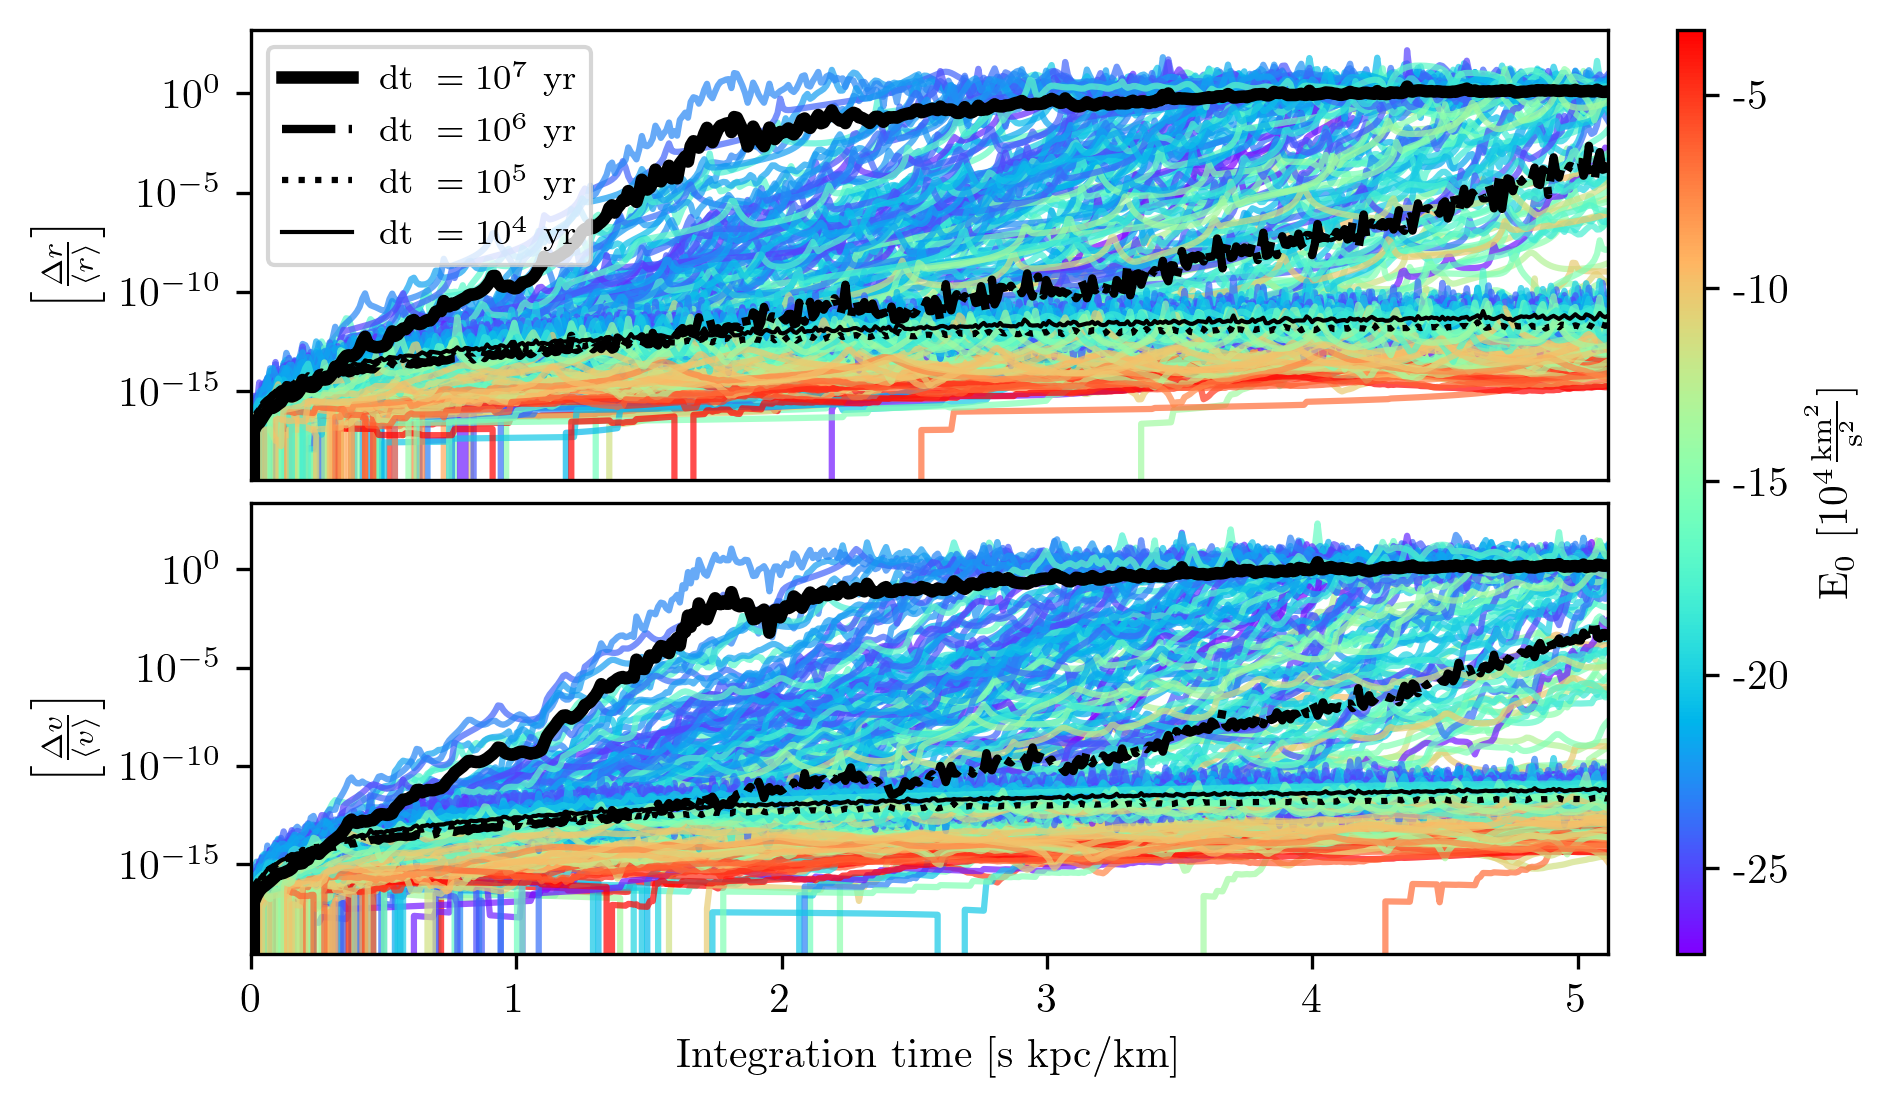
\includegraphics[width=\linewidth]{images/numericalErrorReverseIntegration.png}
            \caption[Time-reversability of the globular cluster system]{The \textit{time-reversability} of the Leapfrog scheme for the 165 Galactic globular cluster's for four different timesteps indicated in the legend. The whole system is only shown for $10^4$~yr and $10^7$~yr to avoid clutter. The clusters are color-coded to their initial orbital energy just as Fig.~\ref{fig:numericalErrorLeapfrogVanilla}}
            \label{fig:numericalErrorReverseIntegration}
        \end{figure}

        Computation time is quite important. Fig.~\ref{fig:numericalErrorGlobularClustersComputationTime} presents the total computation time of integrating the globular cluster system, and the time of a single integration step, which is computed by normalizing the total time by the number of objects and number of steps taken: $T_{\mathrm{total}}/N_{\mathrm{GCs}}/N_{\mathrm{steps}}$. In general, the relationship is linear and the integration time per step per object is roughly constant. The downward trend presented in Fig.~\ref{fig:numericalErrorGlobularClustersComputationTime} is in part a coincidence, as some time realizations minimize this, and in part due to the overhead computation time with initializing and finalizing the calculation contributes less and less with increasing integration time. Nonetheless, for this processor (Apple M2 processor), for a single integration step the mean time is $\sim$ 128~nanoseconds. 
        \begin{figure}
            \centering
            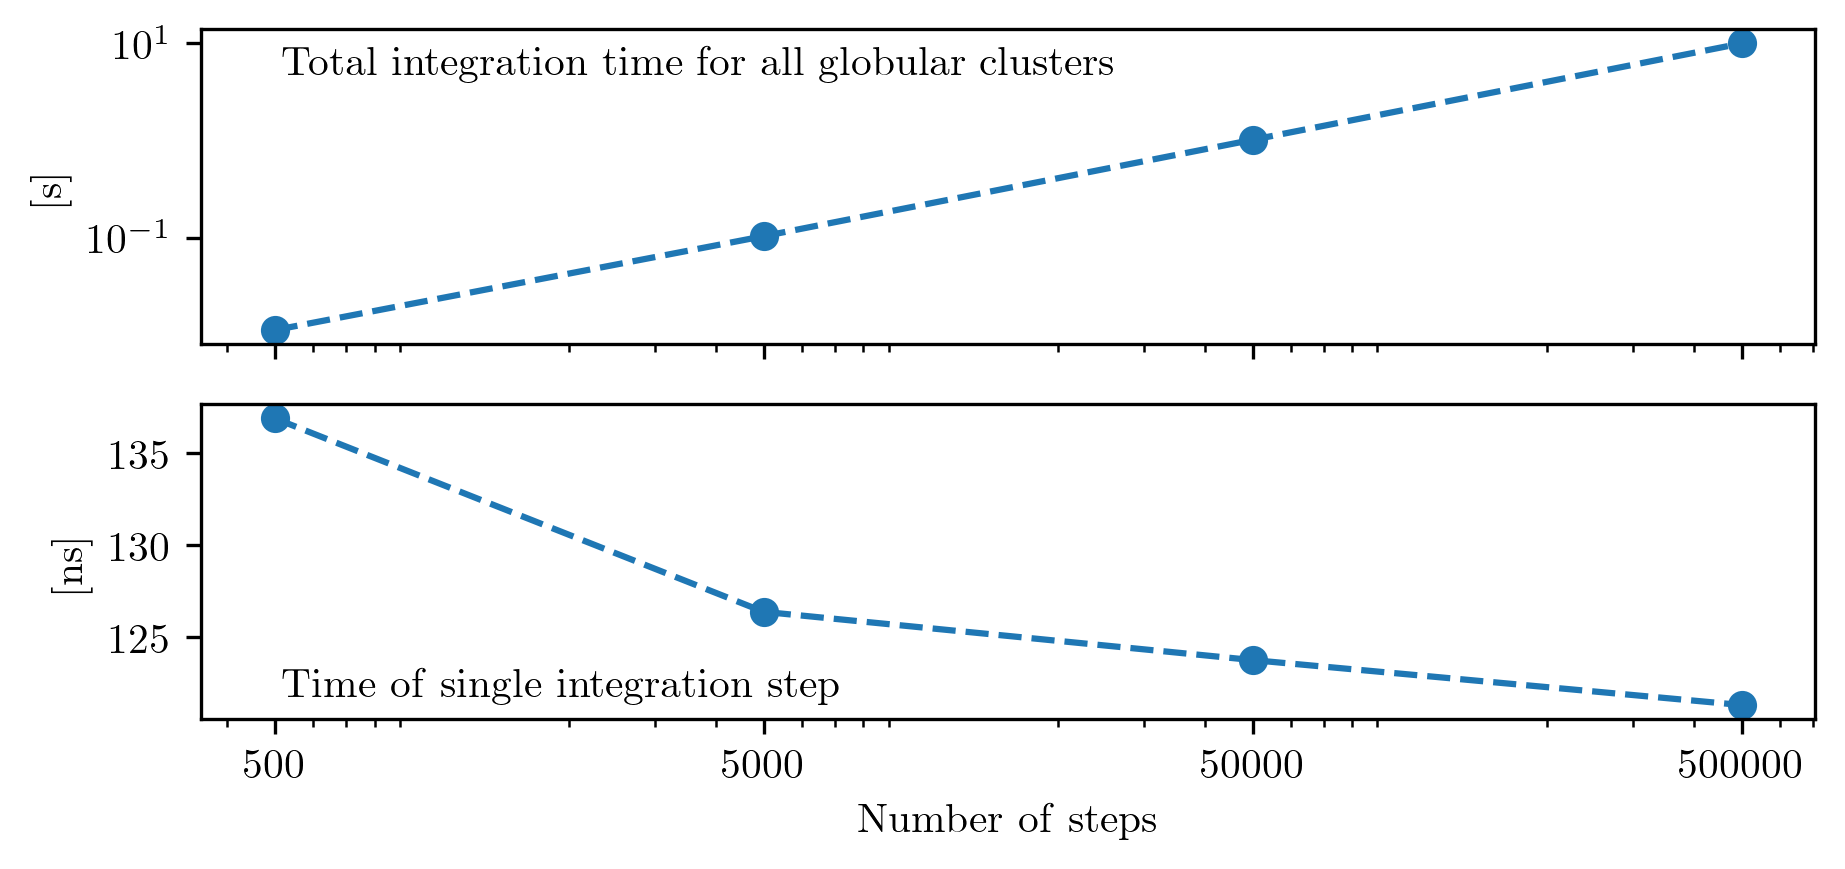
\includegraphics[width=\linewidth]{images/numericalErrorGlobularClustersComputationTime.png}
            \caption[Scaling of the computation time with the number of timesteps]{Computation time for integrating the entire globular cluster system using the Leapfrog scheme. The top panel shows the total time while the bottom shows computation time for a single step, for a single object being integrated. This was performed on a 2022 MacBook Air with an Apple M2 processor. }
            \label{fig:numericalErrorGlobularClustersComputationTime}
        \end{figure}

        The Ruth-Forest algorithm discussed in the previous section was implemented and is reported in Fig.~\ref{fig:numericalErrorRuthForest}. Here, as expected, we see that the percision greatly increases when decreasing the timestep. However, since there are four force evaluations for the for a single timestep, this method is naturally slower per step than Leapfrog. How do the two methods compare over all?
        \begin{figure}
            \centering
            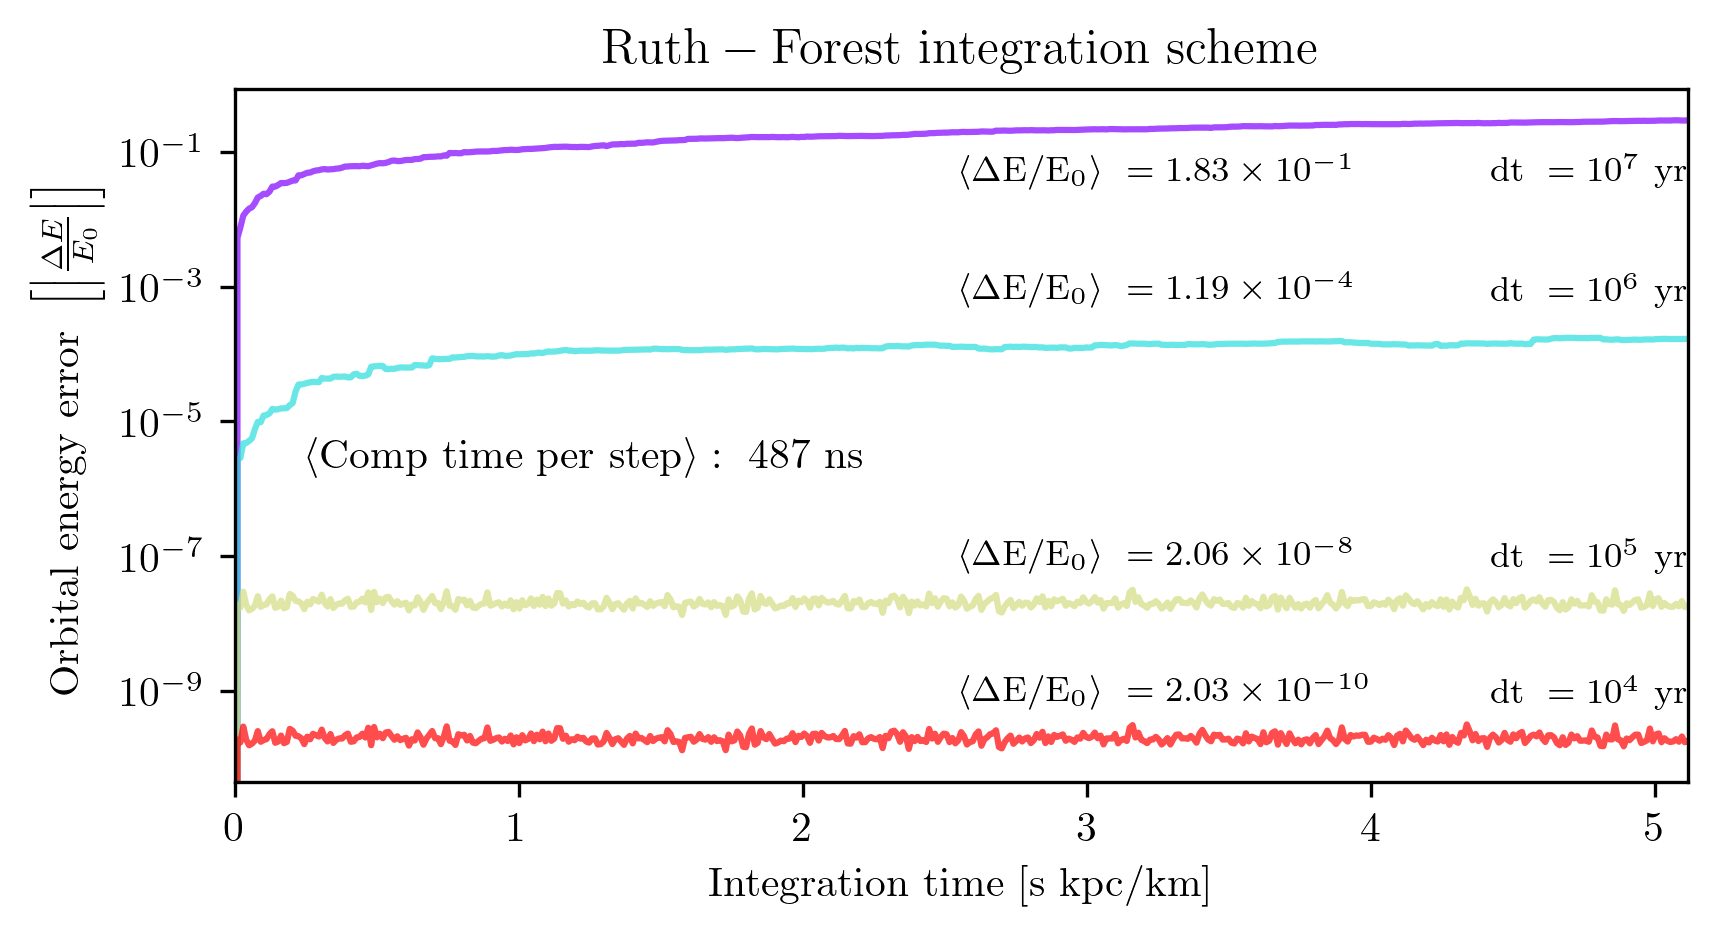
\includegraphics[width=\linewidth]{images/numericalErrorRuthForest.png}
            \caption[Relative orbital energy using the Ruth-Forest scheme]{The conservation of energy error for the Ruth-Forest integration scheme for the globular cluster system. This plot is similar to Fig.~\ref{fig:numericalErrorLeapfrogVanilla}, but does not preesnt on the whole globular cluster system, just the average error in energy for the whole system with a given timestep. The timestep and time-average numerical error for the whole system is presented next to each curve. The average computation time per integration step per single object is as well.}
            \label{fig:numericalErrorRuthForest}
        \end{figure}
        Fig.~\ref{fig:numericalErrorMeanEnergyErrorRuthForestLeapfrog} compares the numerical error for again the total number of steps (which is inversely propertial to the timestep). It is clear that for a given step size, the Ruth-forest outperforms the Leapfrog, but is it actually better? To answer this question, I fit the two curves with their own trend lines to find the number of steps required to have a relative error of $10^{-8}$. With this requirement, The Leapfrog sceme requires 262,641 steps while the Ruth-Forest scheme requires 102,773 steps. However, given the difference in computation time per step, on average, the Forest-Ruth scheme takes $\sim 1.5$x more time for the same degree of numerical precision than the Leapfrog. For this reason, we use the Leapfrog algorithm. In this problem, numerical uncertainties are must less of a limiting factor compared to modeling uncertainties and observational uncertainties, so a better integrator for numerical precision is not worth the pay off of longer computation times. 
        \begin{figure}
            \centering
            \includegraphics[width=\linewidth]{images/numericalErrorMeanEnergyErrorRuthForestLeapfrog.png}
            \caption[Relative orbital energy comparison between leapfrog and Forest-Ruth]{The time averaged error in the conservation of energy for the entire globular cluster system for four different timesteps, for two different integration techinques: the Leapfrog against the Ruth-Forest. Their respective trend lines are shown.}
            \label{fig:numericalErrorMeanEnergyErrorRuthForestLeapfrog}
        \end{figure}

    \subsection{Star-particles in a static globular cluster}

        \begin{verbatim}
        VIDEO: cluster_showing_scale_and_dynamical_time.mp4
        \end{verbatim}
        
        A classic challenge in astronomy and the physical sciences arises when a problem involves two or more physical processes that operate on very different time scales. This is certainly the case when studying globular clusters. Figure~\ref{fig:GCsystemCharacteristicTimes} illustrates the orders-of-magnitude differences in time scales both across the globular cluster population and within individual clusters.

        \begin{figure}
            \centering
            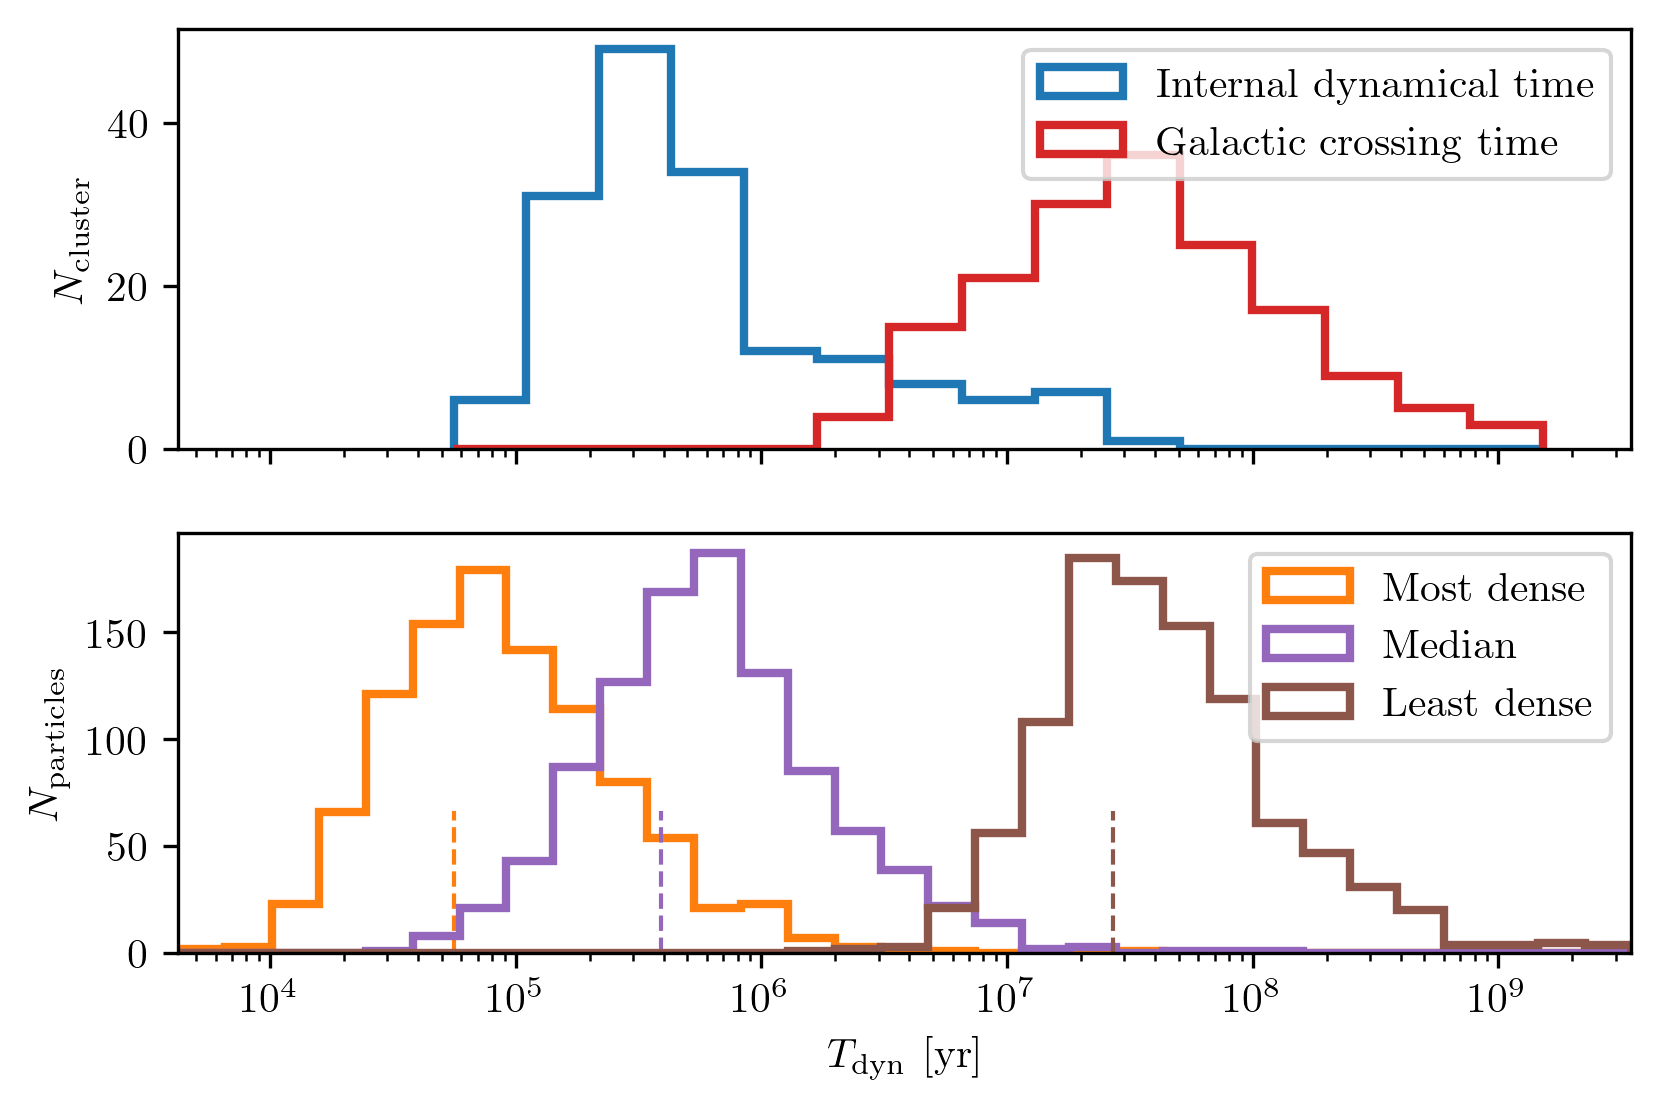
\includegraphics[width=\linewidth]{images/GCsystemCharacteristicTimes.png}
            \caption[Distributions of various dynamical times]{The top panel shows orbital characteristic times of the globular cluster system, while the bottom panel shows internal characteristic times for three selected clusters. \textit{Top}: The red distribution shows the orbital crossing time of each cluster within the Galaxy, while the blue distribution shows a characteristic internal dynamical time. \textit{Bottom}: The distribution of crossing times for 1,000 sampled star particles within the globular clusters with the smallest, median, and largest internal dynamical times. The vertical dashed lines mark the characteristic internal dynamical times.}
            \label{fig:GCsystemCharacteristicTimes}
        \end{figure}

        A useful metric for characterizing a system's time scale is the \textit{crossing time}, which is the time it would take a star to reach the center of the system given its current speed:
        \begin{equation}
            t_\mathrm{cross} = \frac{r}{v}.
        \end{equation}
        While this quantity is not an integral of motion and varies as a star moves, it still provides a convenient and informative estimate of the dynamical time scale. It breaks down in extreme cases, such as a purely radial orbit near pericenter or apocenter where the instantaneous velocity approaches zero, but such cases are rare and do not undermine its utility. We compute the crossing time for each globular cluster in the galaxy (red distribution in the top panel of Fig.~\ref{fig:GCsystemCharacteristicTimes}) as well as for each individual star particle within the clusters.


        For the cluster as a whole, a robust characteristic dynamical time can be defined as:
        \begin{equation}
            \tau = \sqrt{\frac{a^3}{GM}},
        \end{equation}
        where \( a \) is a characteristic size of the system. This is often taken to be the half-mass radius. In this work, I adopt the half-mass radius rather than the Plummer scale radius, though the two are related by \( r_{\mathrm{1/2}} \approx 1.3a \). This time scale was computed for each cluster and is shown as the blue distribution in the top panel of Fig.~\ref{fig:GCsystemCharacteristicTimes}.

        Note that the distribution of cluster dynamical times has a long tail toward longer values, overlapping with the galactic crossing times. A natural question arises: could any cluster have a longer internal dynamical time than its orbital crossing time? The answer should be \textit{no}. If it takes longer for stars to orbit within the cluster than for the entire cluster to orbit the Galaxy, the cluster is effectively unbound or fully disrupted. I examined this question for the Galactic globular cluster population, and the results are shown in Fig.~\ref{fig:GCsystemStabilityDynamicalTimeRatios}. As expected, all clusters have internal dynamical times shorter than their orbital crossing times.

        Interestingly, the ratio of these two time scales serves as a useful diagnostic of cluster stability. Clusters in which stars complete hundreds or thousands of internal orbits per galactic orbit are significantly more stable than those where stars complete only a few. 
        \begin{figure}
            \centering
            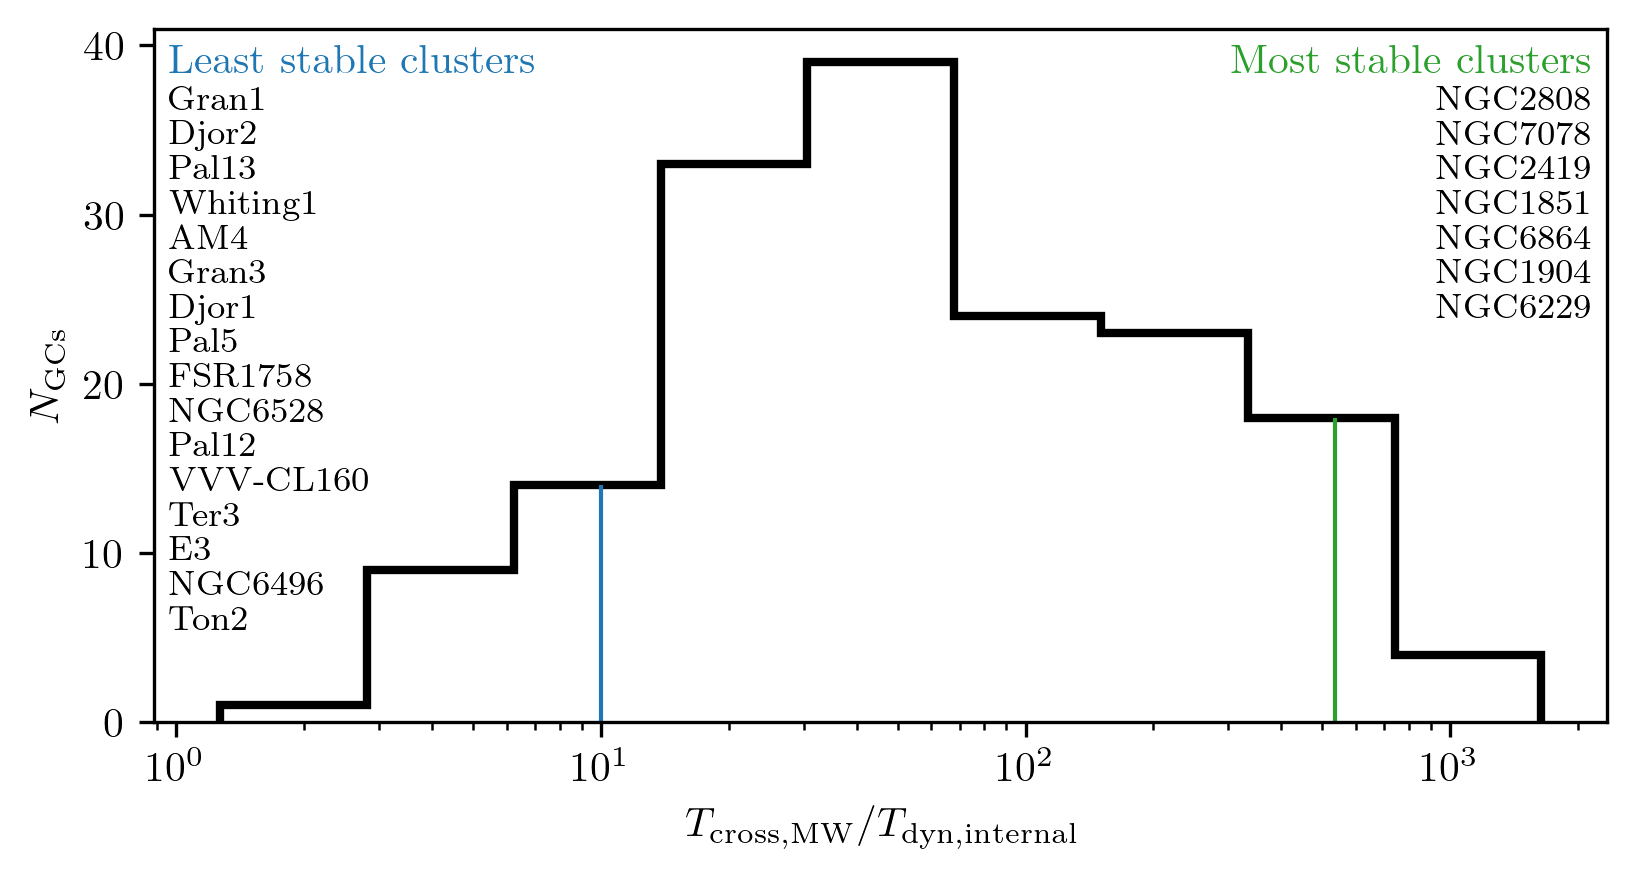
\includegraphics[width=\linewidth]{images/GCsystemStabilityDynamicalTimeRatios.png}
            \caption[Ratio of the globular clusters' internal dynamical times to their Galactic crossing time.]{Ratio of each globular cluster's galactic crossing time to its internal dynamical time (as shown individually in the top panel of Fig.~\ref{fig:GCsystemCharacteristicTimes}). Clusters whose internal dynamical times approach their galactic crossing times are near disruption. In contrast, denser clusters with much shorter internal times are more stable. The vertical bars indicate selected thresholds. Both lists rank clusters by increasing stability, with Gran~1 being the least stable and NGC~6229 the most.}
            \label{fig:GCsystemStabilityDynamicalTimeRatios}
        \end{figure}
        
        To properly compute the orbits of the star particles, the timestep must be small enough to resolve the orbit accurately while the star is inside the cluster. How should we choose this timestep? There are two criteria. The first is that the timestep should be some fraction of the cluster's dynamical time:
        \begin{equation}
            \Delta t' = \alpha ' \tau.
        \end{equation}
        I use a prime to indicate that this is a trial timestep, since the second criterion must also be satisfied: the total number of timesteps should be an integer, 
        \[
            N = \left\lceil \frac{T}{\alpha' \tau} \right\rceil,
        \]
        where $T$ is the total integration time. We round $N$ up to ensure a slightly smaller timestep, which becomes $\Delta t = T/N$. This also redefines the effective timestep fraction as $\alpha = \Delta t / \tau$.

        In the experiments presented in this section, I choose several fractions of each cluster's dynamical time and examine the resulting numerical errors. To efficiently explore a wide range of $\alpha$, I begin with a few trial values of $\alpha'$ and then round the number of steps down so that $N$ is not only an integer, but also a power of two. This leads to the following condition:
        \begin{equation}
            N = 2^{k-1}
        \end{equation}
        where $k \in \mathbb{N}$ is an integer index. The expression for $k$ becomes:
        \begin{equation} 
            k = \left\lceil \log_2\left(\frac{T}{\alpha '  \tau_\mathrm{dyn}}\right) + 1  \right\rceil.
            \label{eq:binary_time_step_criterion}
        \end{equation}
        
        The goal is now to determine the appropriate value of $\alpha$ to ensure energy conservation and time-reversibility. In the analysis presented in the previous sections, I selected timesteps without explicitly relating them to the crossing times of globular cluster orbits. Fig.~\ref{fig:numericalErrorLeapfrogVanilla} shows that a timestep of $\Delta t = 10^4~\mathrm{yr}$ achieves a mean relative energy error of $10^{-8}$. Meanwhile, Fig.~\ref{fig:numericalErrorReverseIntegration} shows that a timestep of $\Delta t = 10^5~\mathrm{yr}$ already achieves convergence in time-reversibility. Comparing these values to the typical crossing time shown in Fig.~\ref{fig:GCsystemCharacteristicTimes}, we find that they correspond to $\alpha$ values of approximately $2 \times 10^{-4}$ and $2 \times 10^{-3}$, respectively.

        In Fig.~\ref{fig:numericalErrorStaticPlummerSphereEnergyError}, I investigate energy conservation in a static Plummer sphere using trial values of $\alpha \in [10^{-4}, 10^{-3}, 10^{-2}, 10^{-1}, 1, 2]$. This experiment shows that values of $\alpha < 10^{-2}$ yield excellent energy conservation. In this section, we do not consider the time-reversability as the previous section has shown the integrations robustness with regard to this metric. However, this is our main metric for the next section.

        \begin{figure}
            \centering
            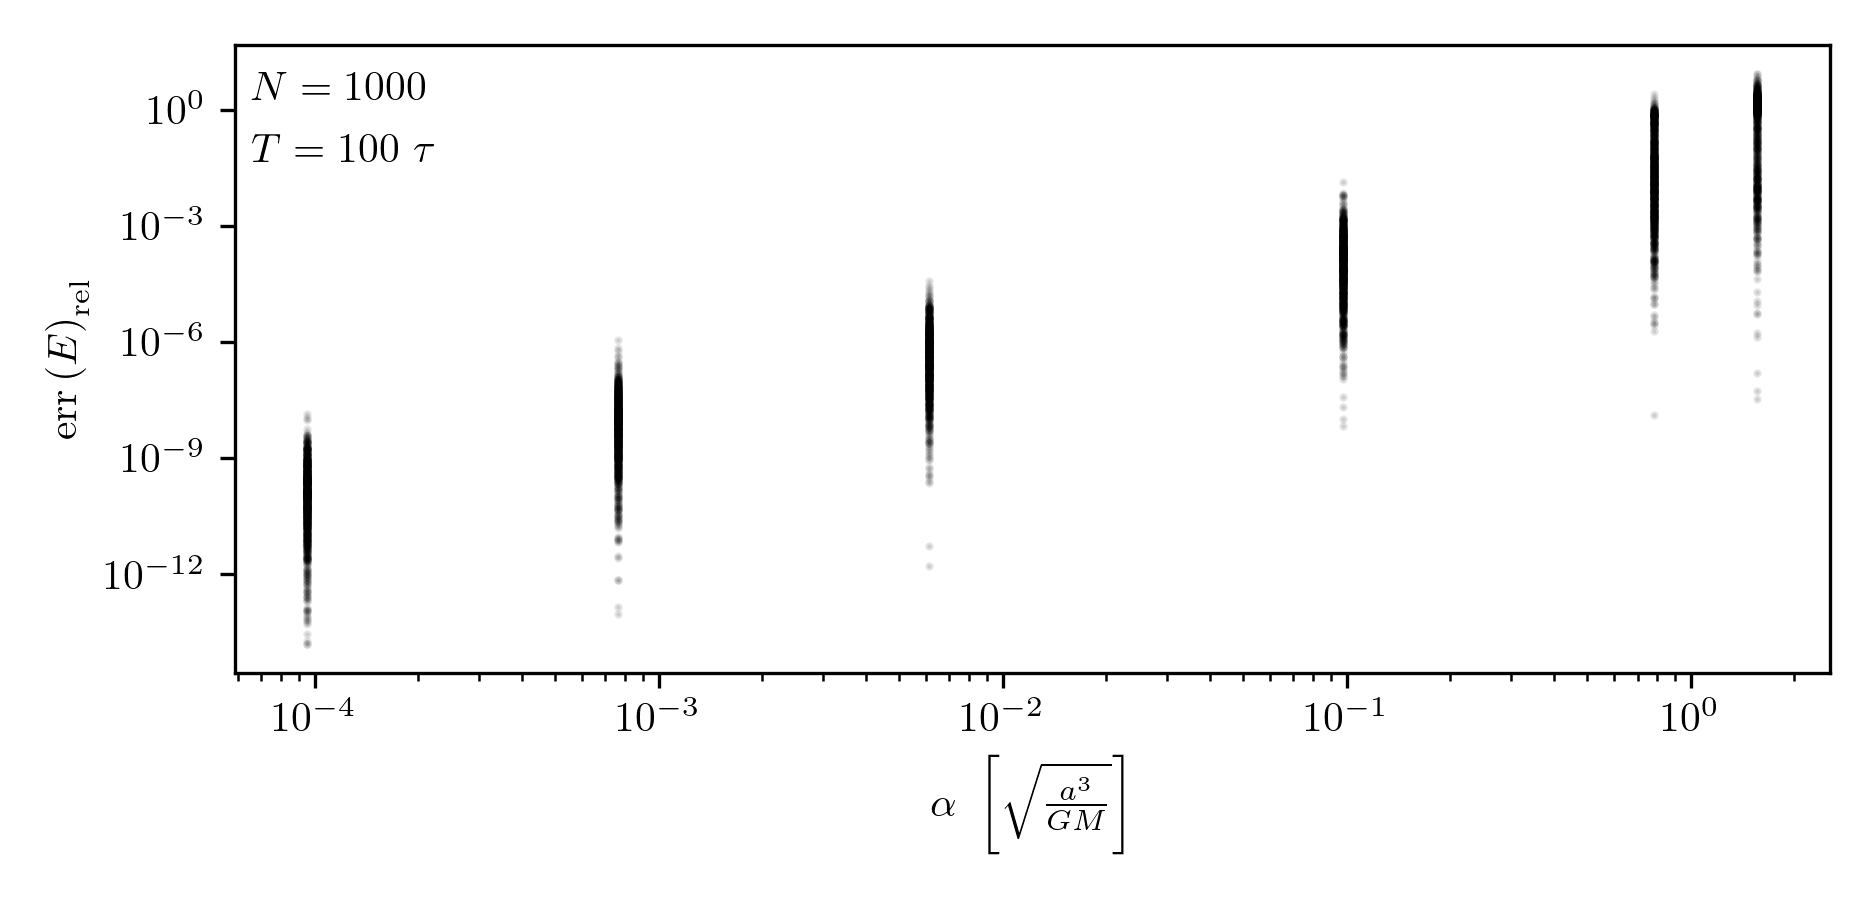
\includegraphics[width=\linewidth]{images/numericalErrorStaticPlummerSphereEnergyError.png}
            \caption[Relative orbital energy for an isolated Plummer sphere]{Relative orbital energy for an isolated Plummer sphere evolved with different timesteps. Each model contains the same number of particles, $N_p$, and is integrated for the same duration, $T$, as indicated on the plot. The x-axis shows the timestep size $\alpha$, defined as a fraction of the internal dynamical time $\tau = \sqrt{a^3 / GM}$.}
            \label{fig:numericalErrorStaticPlummerSphereEnergyError}
        \end{figure}

    \subsection{Full stream generation}
        The preceding sections assessed the numerical stability of integrating globular cluster orbits within the Milky Way, focusing on time-reversibility and relative energy error across two integration schemes: Leapfrog and Forest-Ruth. I also considered the computational cost associated with different temporal resolutions. Separately, I evaluated the energy conservation for star particles evolving within a stationary Plummer sphere, quantifying the relative error as a function of timestep. In that context, the cluster's potential was scaled to its scale radius, mass, and the gravitational constant. This non-dimensionalization allowed me to select timesteps as fractions of the internal dynamical time $\tau$ of each cluster. 

        In this section, I combine them: I examine the quality of orbit integration for star particles evolving within a globular cluster, which in turn is orbiting in the Galactic potential.

        I restrict the analysis here to the Leapfrog integrator for two main reasons. First, although the Forest-Ruth scheme achieves better energy conservation (see Fig.~\ref{fig:numericalErrorMeanEnergyErrorRuthForestLeapfrog}), this comes at a significantly higher computational cost, which outweighs its marginal gains for this application. Second, the equations of motion used to model stream generation require loading the position of the host cluster for each force computation. Because Forest-Ruth evaluates forces at non-uniform substeps, using it would require either: (1) storing and loading the cluster orbit at each substep, which would demand excessive disk space and complex code restructuring; or (2) interpolating the orbit at intermediate times, which introduces ambiguity regarding whether time-reversibility is preserved with linear or cubic interpolation. For these reasons, I opted not to explore Forest-Ruth further in the context of full stream generation.

        To assess the performance of the stream-generation method, I designed a quality assurance experiment, illustrated in Fig.~\ref{fig:NumericalErrorStreamRetrace_NGC6171}. I began by integrating the orbit of a globular cluster's center of mass backward in time by 1~Gyr. At that point, I initialized a Plummer sphere with 512 star particles using the cluster's half-mass radius and total mass. This system was translated to the center-of-mass phase-space coordinates and then integrated forward to the present day, forming a stream. I recorded the resulting positions and computation time. To test time-reversibility, I subsequently integrated the stream particles backward again for 1~Gyr.

        A note on terminology: although the cluster orbit is initialized from present-day observations, in the context of stream generation, I refer to the past position (1 Gyr ago) as the ``initial conditions''. The forward-integrated system represents the ``stream'', and the backward-integrated version of the stream is referred to as the ``retrace''.

        Fig.~\ref{fig:NumericalErrorStreamRetrace_NGC6171} shows the results for four different timesteps. As expected, increasing the timestep degrades time-reversibility. For the largest timestep ($\alpha \approx 1$, top left), the retrace fails to recover the original configuration. The retraced structure remains a stream and does not re-coalesce into a cluster. The results improve rapidly with decreasing timestep: at $\alpha \approx 2 \times 10^{-1}$, most particles return close to their starting positions with only slight offsets. At $\alpha \approx 2 \times 10^{-2}$, nearly all particles recover their initial conditions, and by $\alpha \approx 6 \times 10^{-3}$, the retrace is nearly perfect.

        \begin{figure}
            \centering
            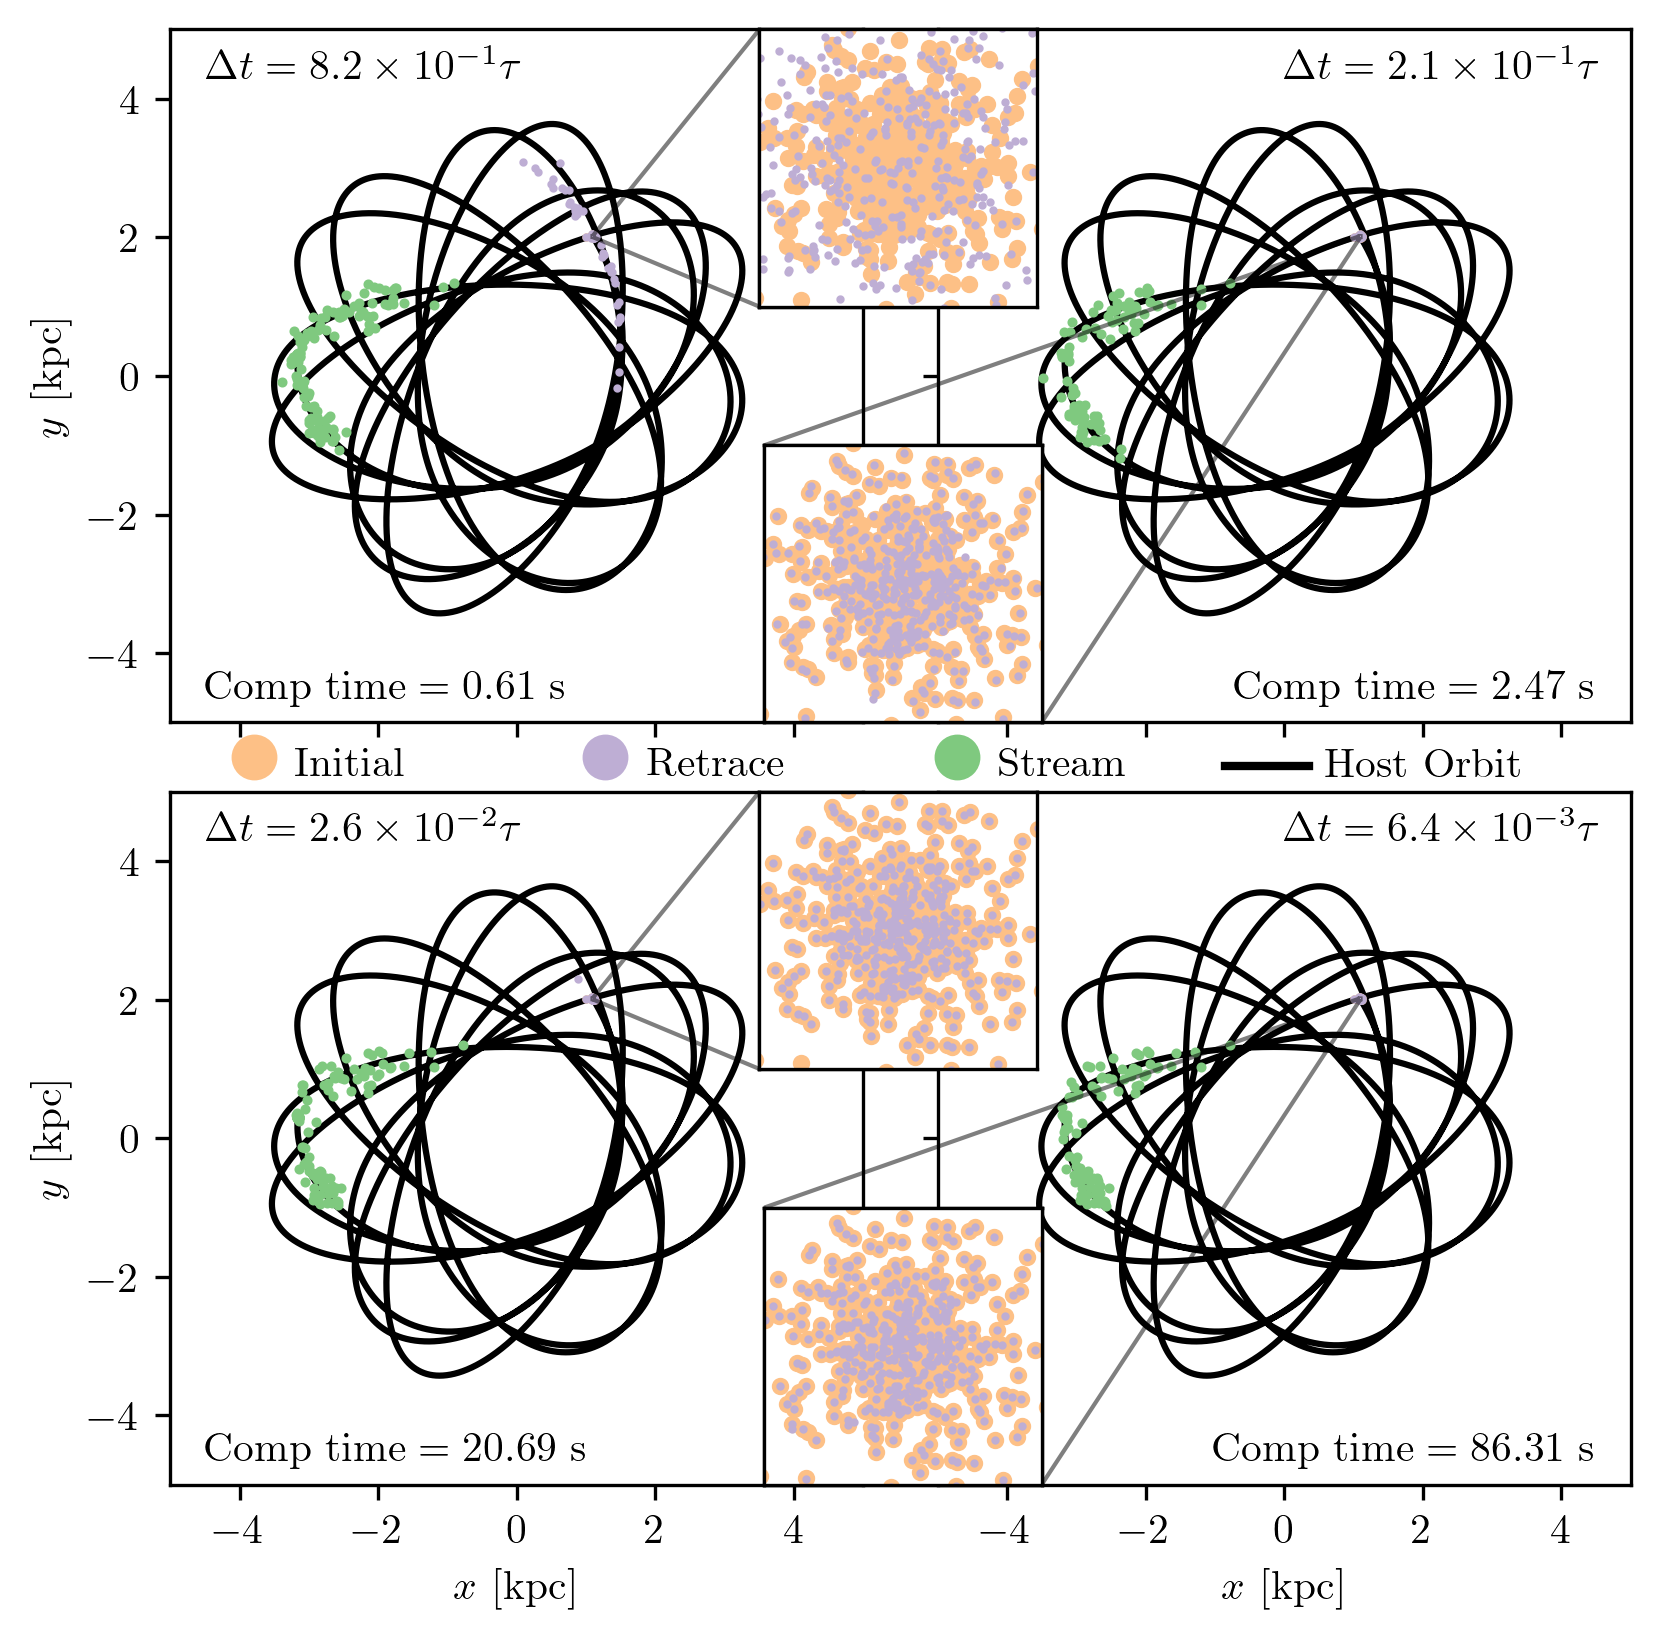
\includegraphics[width=\linewidth]{images/NumericalErrorStreamRetrace_NGC6171.png}
            \caption[Time-reversibility for full stream generation]{Time-reversibility test for NGC~6171. The cluster's orbit was integrated backward by 1 Gyr, and a Plummer sphere of 512 particles was initialized at that position (``Initial''). The system was then integrated forward (``Stream'') and backward again (``Retrace''). Each panel shows a different timestep, which was selected as a fraction of the internal dynamical time $\tau$. The sub-panels zoom in on the cluster core, comparing the initial and retraced positions. Accuracy improves from top to bottom as the timestep decreases.}
            \label{fig:NumericalErrorStreamRetrace_NGC6171}
        \end{figure}

        Fig.~\ref{fig:NumericalErrorStreamRetrace_EnergyErrors} presents the integrator's energy conservation performance during the retrace phase of Fig.~\ref{fig:NumericalErrorStreamRetrace_NGC6171}, across the same timesteps.

        \begin{figure}
            \centering
            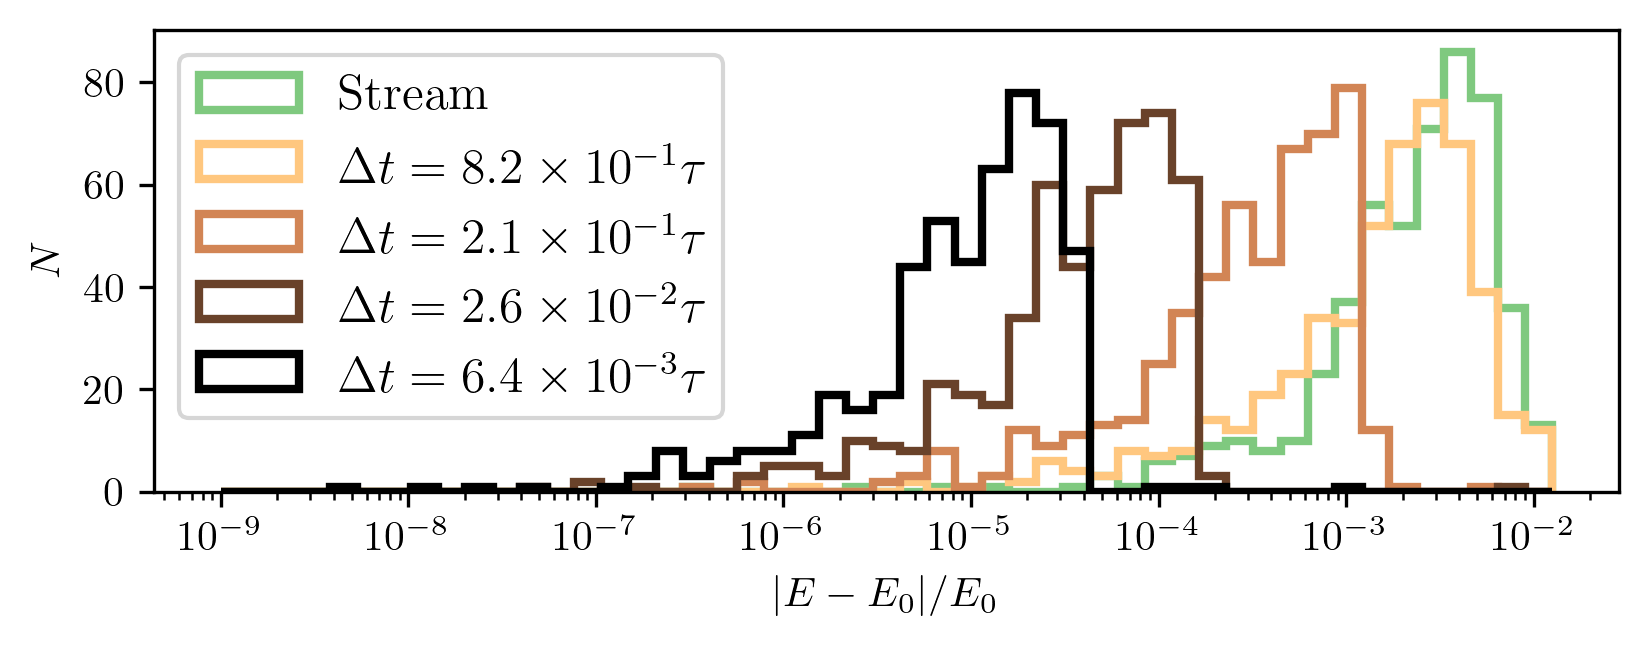
\includegraphics[width=\linewidth]{images/NumericalErrorStreamRetrace_EnergyErrors.png}
            \caption[Relative energy error in retracing full stream generation ]{Relative error in energy conservation during the retrace. As expected, accuracy improves with decreasing timestep. The \textit{stream} distribution shows the final energy of each particle relative to its initial energy and \textit{not} the quality of the integration. This reflects the spread in orbital energies imparted during initial sampling. At large timesteps, the retrace energy distribution approaches that of the stream.}
            \label{fig:NumericalErrorStreamRetrace_EnergyErrors}
        \end{figure}

        Although the retrace fails for the largest timestep in Fig.~\ref{fig:NumericalErrorStreamRetrace_NGC6171}, Fig.~\ref{fig:NumericalErrorStreamRetrace_EnergyErrors} shows that the relative energy error remains modest—between $10^{-4}$ and $10^{-2}$. However, this metric requires careful interpretation. What appears as an ``error'' primarily reflects the intrinsic spread in orbital energies among star particles, relative to the center-of-mass energy. 

        We can estimate this ratio by comparing the internal potential energy scale of the cluster to its orbital energy in the Galaxy. The cluster's characteristic potential is roughly $\Phi \sim GM/a$, with $M \sim 10^5~M_\odot$ and $a \sim 0.005$~kpc, giving $\Phi \sim 10^2~\mathrm{km}^2\,\mathrm{s}^{-2}$. Meanwhile, the typical orbital energy of a globular cluster is around $10^5~\mathrm{km}^2\,\mathrm{s}^{-2}$ (see Fig.~\ref{fig:energy_sensitivity_analysis_MWGCS_to_distance_RV_mu}). 

        This three-order-of-magnitude difference implies that the intrinsic energy spread from the Plummer sampling is about $10^{-3}$ of the total orbital energy, which is consistent with the the apparent energy ``error'' in the stream of Fig.~\ref{fig:NumericalErrorStreamRetrace_EnergyErrors}. Thus, this differences does not arise from numerical drift, but from the physical energy distribution encoded in the initial conditions. 

        Fig.~\ref{fig:NumericalErrorStreamRetrace_NGC6171} \& Fig.~\ref{fig:NumericalErrorStreamRetrace_EnergyErrors} demonstrate the case of a single cluster. How is the energy conservation for the entire catalog? Fig.~\ref{fig:NumericalErrorStreamRetraceEnergyConservation} presents the realtive error in the conservation of energy for retracing the orbit of each individual star particle per globular cluster for each cluster in the catalog. Each data point reports the mean error in the conservation of energy. Each cluster was integrated for 5~Gyr. The upper limits for the timesteps were sampeld logarithmically between $10^{0}$ and $10^{-2}$, the exact timesteps are based on the criterion from Eq.~\ref{eq:binary_time_step_criterion}.

        % From inspecting Fig.~\ref{fig:NumericalErrorStreamRetrace_NGC6171}, a timestep less than $3\times10^{-2}~\tau$ is great for retracing the orbit of each star particle and even $2\times10^{-1}~\tau$ suceeds in generally retracing the cluster. This would place the retrace energy conservation between $10^{-5}-10^{-3}$ on average per system. 
        \begin{figure}
            \centering 
            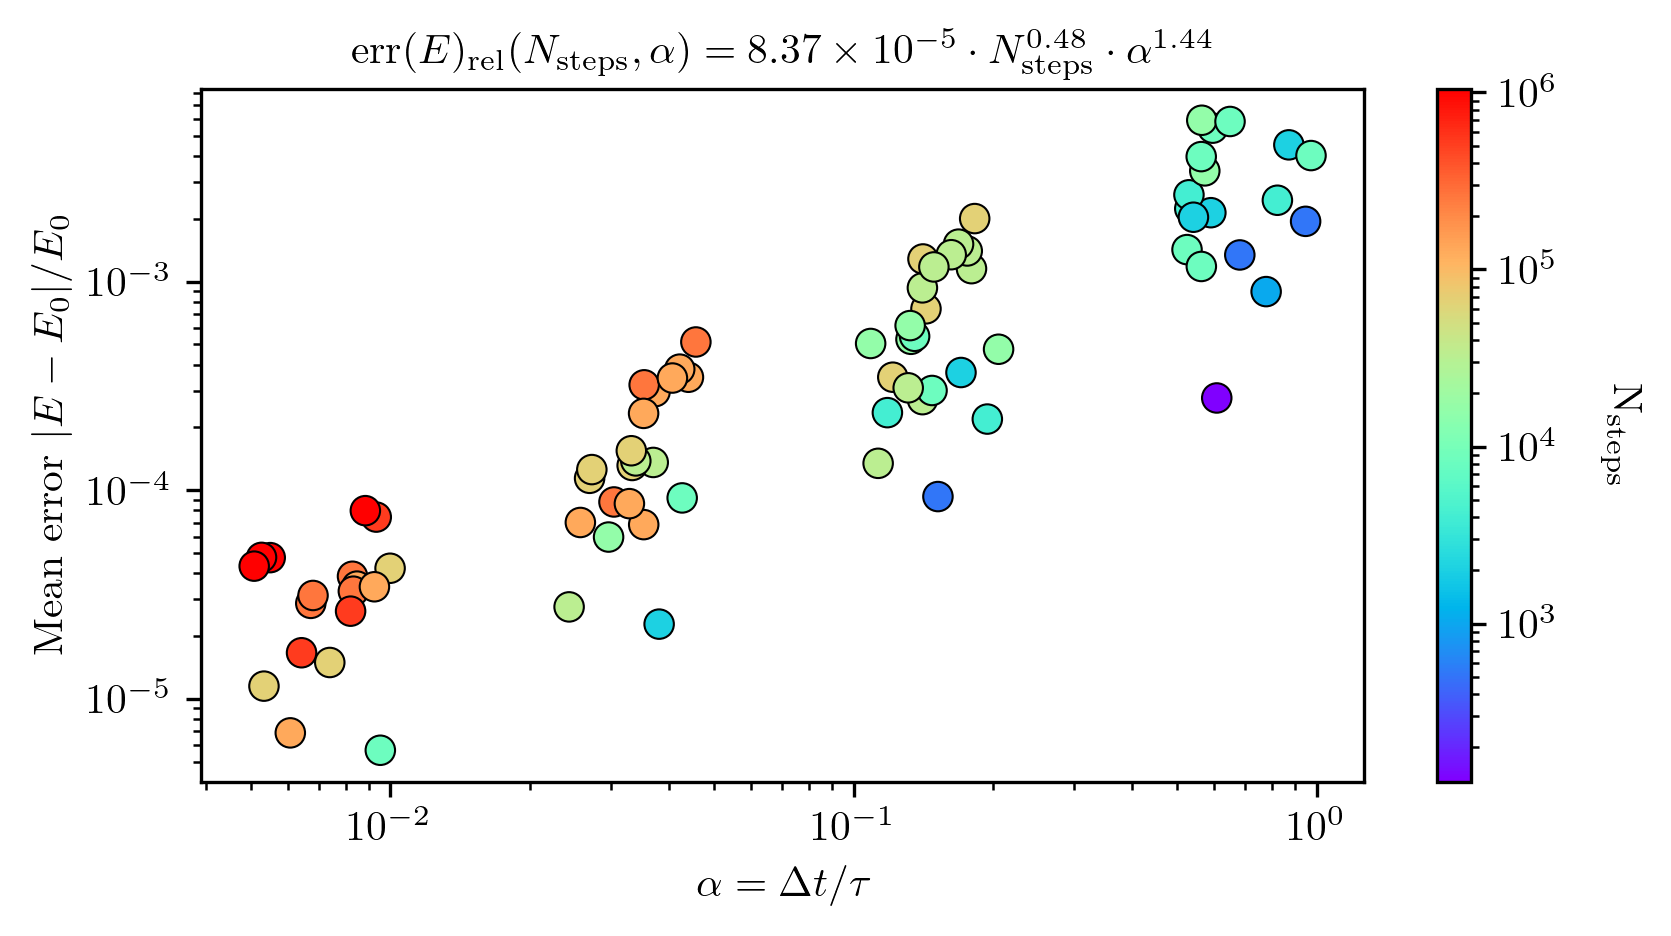
\includegraphics[width=\linewidth]{images/NumericalErrorStreamRetraceEnergyConservation.png}
            \caption[Relative error in energy conservation of stream generation for the whole catalog]{The conservation of energy for the retrace of each globular cluster in the catalog. Each cluster was sampled with 512 particles and integrated for 5~Gyr. Four upper thresholds for each timestep were logarithmically sampled between $10^{0}$ and $10^{-2}$, and selected individually for each cluster in combination with it's internal dynamical time that evenly divided the integration time. }
            \label{fig:NumericalErrorStreamRetraceEnergyConservation}
        \end{figure}

        The quality of the solutions is fundamental for proper results. However, computation time and cost is also very important. The main motivation in using the restricted three body problem was to save computation time. With N~body, the computation time should scale with $N_p^2$, while for the restricted three body problem it should scale with $N_p$. For both, it should scale linearly with the number of integration steps. 

        How does \texttt{tstrippy} perform? Fig.~\ref{fig:NumericalErrorComputationTimeScalingForStreams} presents an the results from an experiment with all the globular clusters, integrating them each for 1~Gyr. I choose the timestep to be at most 1/20 of each internal dynamical time, thus since each cluster has a different dynamical time, it will require a different number of steps. For each of these tests I use $10^1,~10^2,~10^2,~10^3$ particles and launched them on cluster at the paris observatory. Then, I fit a scaling law of $C(N_p,N_s) = \langle C\rangle N_p^a N_s^b$. If the code scales linearly, then each exponent, $a,~b$, should be 1 and $\langle C\rangle$ would be the mean computation time. 
        
        Fig~\ref{fig:NumericalErrorComputationTimeScalingForStreams} shows that the code is \textit{less} efficient than linear scaling with number of particles, since the best fit exponent is $1.35$. However, it scales \textit{better} than linear with the number of steps. Perhaps this can be explained by the fact that there is overhead time involved for initiating and ending each simulation. As the number of steps increases the fixed overhead proportionally takes up less of the total time. Since the power law has an exponent of $0.95$, the overhead is marginal. However, it is fortunate that the exponent is not greater than 1, which would mean the code would slow down with execution time. 
        \begin{figure}
            \centering
            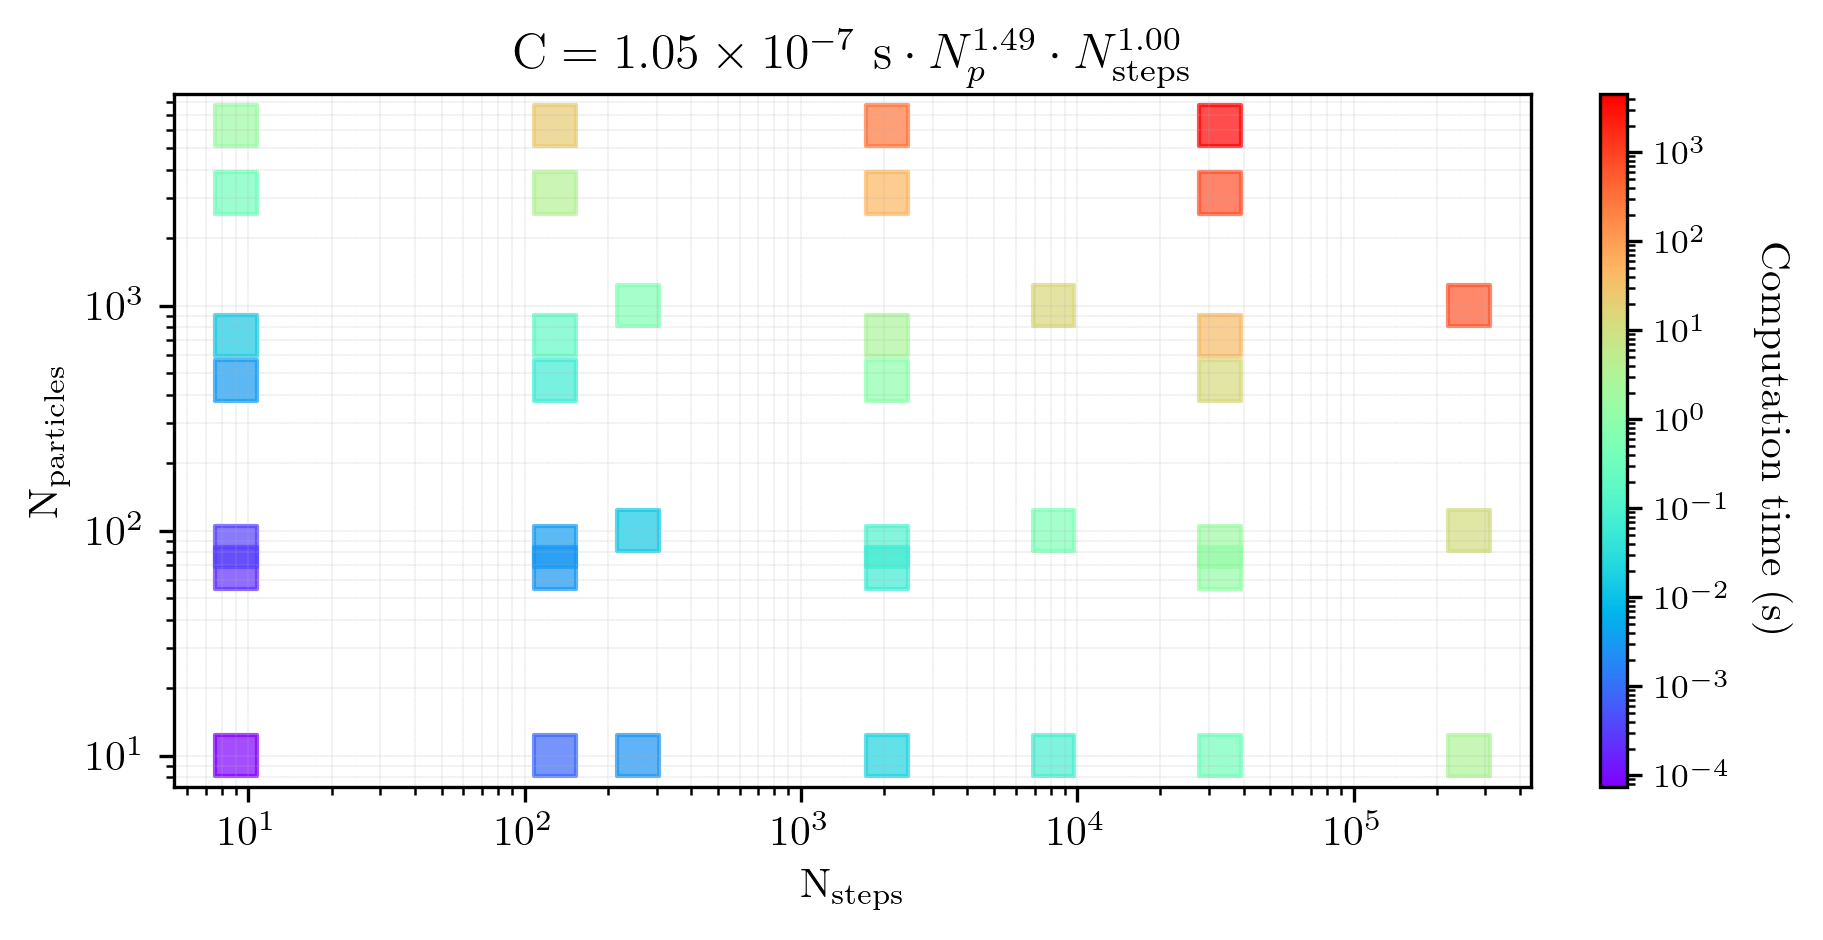
\includegraphics[width=\linewidth]{images/NumericalErrorComputationTimeScalingForStreams.png}
            \caption[Profiling \texttt{tstrippy}'s computation time for the number of particles and time steps]{How the computation scale time scales with the number of particles and the number of steps taken.}
            \label{fig:NumericalErrorComputationTimeScalingForStreams}
        \end{figure}
        Putting Fig.~\ref{fig:NumericalErrorStreamRetraceEnergyConservation} and Fig.~\ref{fig:NumericalErrorComputationTimeScalingForStreams} together, we get can estimate for how long it completes to run these simulations. If we want all simualtions to have error better relative error on the retraced conservation of energy than about 10$^{-3}$, then we must pick timesteps that are smaller than about 1/20 of the dynamical time. With this criteria selected, we can compute the number of timesteps necessary for each globular cluster, which is a function of it's internal dynamical time. By doing so, I find that the fastest cluster can be computed in $\sim$~30~minutes. The median computation time is $\sim$17~hours. The largest computation time was $\sim$~5~days. The total CPU time for the whole catalog is $\sim$~194~days. 

        \subsubsection{A note on non-symplectic integration}

        During the writing of this thesis, I discovered a bug in my code that affected the integration scheme. Specifically, the error concerned the way I handled the host orbit during the integration of the star particles. In earlier implementations, I would integrate the orbit of the host using the same timestep that I used later to integrate the orbits of the star particles. However, this approach violated the structure of the Leapfrog integration scheme.

        In Hamiltonian integration, it is essential that the drift and kick steps alternate in a consistent manner. Since I implemented a \textit{drift}-\textit{kick}-\textit{drift} (DKD) scheme, the kicks occur at the midpoint of each timestep, meaning that forces should be evaluated at intermediate positions. Previously, I erroneously computed the relative position vector as
        \[
        \Delta \vec{r}_i = \vec{r}_{p,i+1/2} - \vec{r}_\mathrm{GC,i},
        \]
        instead of the correct expression:
        \[
        \Delta \vec{r}_i = \vec{r}_{p,i+1/2} - \vec{r}_\mathrm{GC,i+1/2}.
        \]

        This mistake appeared in both \citet{2023A&A...673A..44F} and \citet{2025A&A...699A.289F}. Does this invalidate our results? To assess the impact, we can compare Figs.~\ref{fig:NumericalErrorStreamRetrace_Pal5_Nsteps_32768_stepsPerTau_420} and \ref{fig:NumericalErrorStreamRetrace_NGC6171_Nsteps_1048576_stepsPerTau_311}. In Fig.~\ref{fig:NumericalErrorStreamRetrace_Pal5_Nsteps_32768_stepsPerTau_420}, the same retracing experiment was performed, but using the flawed integration: the host orbit was only provided at the same grid points as the stream. In the left panel, we see that the globular cluster does not perfectly re-coalesce when integrating backward in time, but the result is not catastrophic. Physically, we do not expect this process to be perfectly time-reversible; however, such irreversibility should ideally arise from physical modeling, not from numerical artifacts.

        We also observe that the distribution of the relative error in energy conservation is nearly identical between the retraced and the original stream. In any case, once the stars move beyond the Jacobi radius, their dynamics are dominated by the galactic potential. Since this potential was integrated correctly and symplectically, the orbits of stars outside the cluster remain reliable and physically meaningful.

        \begin{figure}
            \centering
            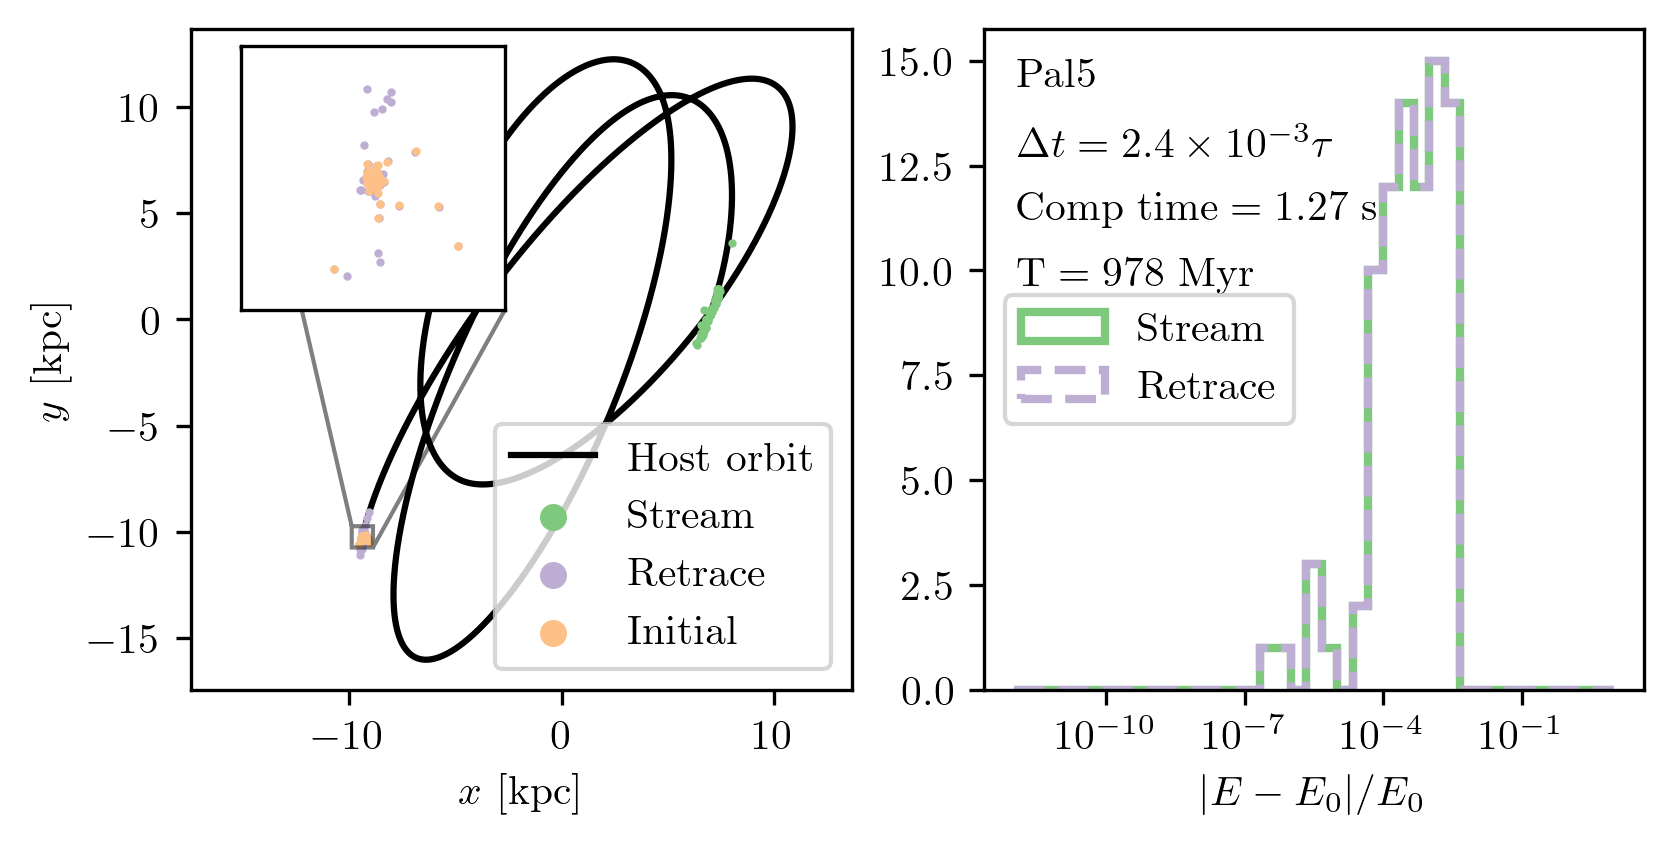
\includegraphics[width=\linewidth]{images/NumericalErrorStreamRetrace_Pal5_Nsteps_32768_stepsPerTau_420.png}
            \caption[An illustration of non-symplectic integration]{An illustration of how an incorrect integration scheme breaks time reversibility. The center of mass of Palomar~5 was integrated backward in time by 1~$\mathrm{s}~\frac{\mathrm{kpc}}{\mathrm{km}}$. A Plummer sphere with 464 particles was sampled around this position (labeled “Initial”), then integrated forward to produce the “Stream.” The right panel shows the distribution of relative energy error. The stream was then integrated backward in time by the same amount, resulting in the “Retrace” configuration. The timestep was chosen as a fraction of the internal dynamical time scale, $\tau$.}
            \label{fig:NumericalErrorStreamRetrace_Pal5_Nsteps_32768_stepsPerTau_420}
        \end{figure}
        As a result of this discovery, I updated the \texttt{tstrippy} code to warn users if the host orbit is not sampled at $2N + 1$ points, where $N$ is the number of integration steps. While the flawed implementation breaks strict symplecticity for the internal cluster dynamics, the Leapfrog integration for the globular cluster orbits was still used correctly. This ensures that the cluster center of mass returns to its present-day sky position and that stars outside the cluster follow accurate galactic orbits. Ultimately, the simplification of using a static Plummer sphere—whose mass and size remain fixed—is a greater limitation than this particular numerical error.

        Lastly, I discovered this error while writing about the Forest-Ruth integration method. To implement this scheme correctly, I would need to know the position of the globular cluster's center of mass at four intermediate points across two timesteps, with the spacing determined by the coefficients in Table~\ref{tab:forest_ruth_coeffs}. This would require either storing additional mini-time-step data or interpolating the globular cluster's trajectory between saved snapshots. Both options would necessitate a substantial refactoring of the code or an impractical increase in memory usage per orbit. Given the results shown in Fig.~\ref{fig:numericalErrorMeanEnergyErrorRuthForestLeapfrog}, the gain in accuracy does not justify the computational cost.


\section{Tstrippy}
    This project is built on \texttt{f2py}, which allows integration between Fortran and Python. The core motivation behind this choice is performance: Fortran, as a compiled language, provides significantly faster execution for numerically intensive tasks, while Python—especially within Jupyter notebooks—offers a convenient environment for development, experimentation, and visualization. \texttt{F2py} stands for \textit{Fortran to Python} \citep{peterson2009f2py}, and it is included as a module within NumPy \citep{numpy_f2py_manual,2020Natur.585..357H}. The name of the project, \texttt{tstrippy}, stands for \texttt{T}idal \texttt{Strip}ping in \texttt{Py}thon.

    \texttt{F2py} supports Fortran 77, 90, and 95 standards, so we chose to write the code in Fortran 90 to make use of \textit{modules}. In Fortran, a module encapsulates data and subroutines in a manner somewhat analogous to classes in object-oriented programming. However, Fortran modules do not support inheritance, and only a single instance of a module can exist at a time—unlike classes, which can be instantiated multiple times.

    \texttt{Tstrippy} package is structured around five core Fortran modules, each responsible for a distinct aspect of the simulation:
    \begin{itemize}
        \item \texttt{integrator}: This is the central module of the code. It stores particle positions and velocities, computes forces, and evolves the system forward in time. It also handles the writing of output data at specified intervals and interfaces with all other modules in the code.
        \item \texttt{potentials}: This module defines the analytical potentials used to compute gravitational forces. It currently supports several models, including \texttt{Plummer}, \texttt{Hernquist}, \texttt{AllenSantillian}, \texttt{MiyamotoNagai}, the bar model \texttt{LongMuraliBar} from \citet{1992ApJ...397...44L}, and the composite model from \texttt{pouliasis2017pii} \citep{2017A&A...598A..66P}. This module can also be called in Python, allowing users to call potential functions directly, e.g., for computing energies during post-processing.
        \item \texttt{hostperturber}: This module handles the host globular cluster. It stores its orbit (i.e., timestamps, positions, and velocities) and ensures its synchronization with the simulation's internal clock. It computes the gravitational influence of the host cluster on each star particle. This is an internal module only.
        \item \texttt{perturbers}: Similar in function to \texttt{hostperturber}, this module supports additional perturbing clusters. It allows for the inclusion of multiple perturbers and computes their collective force on each particle. If object-oriented programming were available in Fortran, both this module and \texttt{hostperturber} would naturally inherit from a shared parent class. This module only uses the positions, masses, and characteristic radii of the other perturbers. The velocities are not imported.
        \item \texttt{galacticbar}: This module stores parameters for the Galactic bar, including the polynomial coefficients for its angular displacement as a function of time:
        \[
        \theta(t) = \theta_0 + \omega t + \dot{\omega} t^2 + \ddot{\omega} t^3 + \dots
        \]
        If a user wants a bar with a constant rotation speed, then they may pass two coefficients. If they want a bar that accelerates for decelerates, they may mass more coefficients for the higher order terms. The module performs transformations into the rotating bar frame, computes the forces in that frame, and then transforms the forces back to the Galactocentric reference frame.
    \end{itemize}
    This modular structure makes it straightforward to extend the code by adding new physics in the form of additional modules.

    To make the package installable and easy to distribute, I initially followed the guide by \citet{pythonpackagingguide}, which describes how to create a Python package using \texttt{setuptools}—the standard build system in the Python ecosystem. However, compatibility between \texttt{setuptools} and \texttt{f2py} was broken starting with NumPy~$>$~1.22 (released June 22, 2022\footnote{\url{https://github.com/numpy/numpy/releases/tag/v1.22.0}}) and Python~$>$~3.9.18 (released June 24, 2024\footnote{\url{https://www.python.org/downloads/release/}}). This meant that Fortran extensions could only be compiled using deprecated versions of both. These older versions of NumPy were also not compatible with Apple's ARM-based M1 and M2 processors, rendering the code unusable on modern Mac systems.

    This limitation stemmed from the deprecation and eventual removal of \texttt{numpy.distutils}, the tool that previously enabled seamless integration of Fortran code in NumPy-based packages. As of NumPy~1.23 and later, \texttt{numpy.distutils} was deprecated, and with NumPy~2.0, it was removed entirely. The NumPy developers recommended migrating to \texttt{meson} \citep{meson_manual} or \texttt{Cmake}.

    To address these issues, I migrated the build process to \texttt{meson}, a language-agnostic build system capable of compiling Fortran, C, and Python extensions across architectures. This eliminated compatibility problems and made the build process architecture-independent. The build system now automatically detects the system architecture and compiles accordingly.

    The code is fully open source and available on GitHub.\footnote{\url{https://github.com/salvatore-ferrone/tstrippy}} To support users, I created documentation hosted on \texttt{readthedocs.io}\footnote{\url{https://tstrippy.readthedocs.io/en/latest/}}, which includes working examples and basic usage guides. A minimal test suite, written using \texttt{pytest}, is also included. While not exhaustive, the tests ensure that core functionality remains intact as the code evolves. In the next section, I present a minimal example of how the user may use the code within a python script.

    \subsection{Minimum example}
        If the package is properly installed on the system, it can be imported at the top of any Python script:
        \small
        \begin{lstlisting}[language=python]
            import tstrippy    
        \end{lstlisting}
        \normalsize
        Next, the user must load or define the initial conditions. The code provides:
        \begin{itemize}
            \item The masses, sizes, and kinematics of the globular cluster catalog from \citet{2018MNRAS.478.1520B};
            \item The galactic potential parameters for model II of \citet{2017A&A...598A..66P}; and
            \item A galactic reference frame.
        \end{itemize}

        \small
        \begin{lstlisting}[language=python]
            GCdata      = \
                tstrippy.Parsers.baumgardtMWGCs().data
            MWparams    = \
                tstrippy.Parsers.potential_parameters.pouliasis2017pii()
            MWrefframe  = \
                tstrippy.Parsers.potential_parameters.MWreferenceframe()
        \end{lstlisting}
        \normalsize
        The user must then select the system to integrate. For example, to integrate the orbits of observed globular clusters, one must convert the ICRS coordinates to a Galactocentric frame using \texttt{astropy} and the provided MW reference frame. Alternatively, to simulate a star cluster, one can generate a Plummer sphere:
        \small
        \begin{lstlisting}[language=python]
            xp,yp,zp,vxp,vyp,vzp=\
            tstrippy.ergodic.isotropicplummer(G,massHost,halfmassradius,NP)
        \end{lstlisting}
        Here, \texttt{NP} is the number of particles, \texttt{halfmassradius} is the system's half-mass radius, \texttt{massHost} is the total mass of the Plummer sphere, and \texttt{G} is the gravitational constant. All values must be in the same unit system.

        The integrator must then be initialized. All parameters are passed via lists that are unpacked at the function call. Here is an example of initializing the integrator for a stellar stream in a potential that includes a rotating galactic bar:
        \small
        \begin{lstlisting}[language=python]
            tstrippy.integrator.setstaticgalaxy(*staticgalaxy)
            tstrippy.integrator.setinitialkinematics(*initialkinematics)
            tstrippy.integrator.setintegrationparameters(*integrationparameters)
            tstrippy.integrator.inithostperturber(*hostperturber)
            tstrippy.integrator.initgalacticbar(*galacticbar)
            tstrippy.integrator.setbackwardorbit()
        \end{lstlisting}
        \normalsize

        \begin{itemize}
            \item \texttt{setstaticgalaxy} specifies the static potential model and passes its parameters.
            \item \texttt{setinitialkinematics} provides the initial positions and velocities of the particles.
            \item \texttt{setintegrationparameters} defines the initial time, timestep, and number of steps.
            \item \texttt{inithostperturber} specifies the globular cluster's trajectory and mass as a function of time.
            \item \texttt{initgalacticbar} defines a rotating bar. It takes the name of the bar model, potential parameters, and spin parameters.
            \item \texttt{setbackwardorbit} reverses the velocity vectors and sets the internal clock to count down: $t_i = t_0 - i \cdot \Delta t$. For the usecase presented in this work, \texttt{setbackwardorbit} is used for computing the globular cluster orbits and not for the star-particles. 
        \end{itemize}
        The user can choose between two output modes during integration:
        \begin{lstlisting}
            tstrippy.integrator.initwriteparticleorbits(nskip,myoutname,myoutdir)
            tstrippy.integrator.initwritestream(nskip,myoutname,myoutdir)
        \end{lstlisting}
        Conceptually, these represent two output paradigms:
        \begin{itemize}
            \item \texttt{initwriteparticleorbits} saves the full orbit of each particle to an individual file.
            \item \texttt{initwritestream} saves full snapshots of all particles at selected timesteps.
        \end{itemize}
        Both functions take:
        \begin{itemize}
            \item \texttt{nskip}: number of timesteps to skip between outputs;
            \item\texttt{myoutname}: the base file name;
            \item \texttt{myoutdir}: the output directory.
        \end{itemize}
        The output files will be named like: \texttt{../dir/temp0.bin}, \texttt{../dir/temp1.bin}, ..., up to \texttt{../dir/tempN.bin}, where $N = N_\mathrm{step} / N_\mathrm{skip}$. Note that the files are written in Fortran binary format. Although \texttt{scipy.io.FortranFile} can read them, I use a custom parser based on \texttt{numpy.frombuffer} to avoid the SciPy dependency. Once all parameters are set, the user can proceed with integration using one of two methods:
        \subsubsection*{Full orbit integration (in memory)}
        \small
        \begin{lstlisting}
            xt,yt,zt,vxt,vyt,vzt=\
                tstrippy.integrator.leapfrogintime(Ntimestep,nObj) 
            timestamps=\
                tstrippy.integrator.timestamps.copy()
        \end{lstlisting}
        \normalsize
        \texttt{leapfrogintime} stores the full orbit of each particle in memory. This is useful for a small number of particles or short integrations—e.g., rapid parameter studies in a notebook. However, for large simulations it can be prohibitively memory-intensive. For instance, integrating all globular clusters at high time resolution might require:
        \begin{equation}
            7 \times N_p \times N_\mathrm{step} \times 8~\mathrm{Byte} \approx 450~\mathrm{GB}
        \end{equation}
        if $N_\mathrm{step} \approx 10^7$. This will likely exceed system RAM.

        \subsubsection*{Final state only}
        \small
        \begin{lstlisting}
            tstrippy.integrator.leapfrogtofinalpositions()
            xf  = tstrippy.integrator.xf.copy()
            yf  = tstrippy.integrator.yf.copy()
            zf  = tstrippy.integrator.zf.copy()
            vxf = tstrippy.integrator.vxf.copy()
            vyf = tstrippy.integrator.vyf.copy()
            vzf = tstrippy.integrator.vzf.copy()
            finaltime=tstrippy.integrator.currenttime.copy()
        \end{lstlisting}
        \normalsize
        \texttt{leapfrogtofinalpositions()} performs the integration but only returns the final phase-space coordinates. These arrays must be copied before deallocating memory:
        \small
        \begin{lstlisting}
            tstrippy.integrator.deallocate()
        \end{lstlisting}
        \normalsize
        Deallocating is necessary to avoid memory leaks or crashes in Jupyter when rerunning code cells.

    \subsection{Reflection on developing \texttt{tstrippy}}
        The earliest version of this code began as a simple Fortran script built to integrate test particles in specific gravitational potential models. Since I was already familiar with Fortran and had working routines, I chose to build on that foundation, gradually transforming the script into a modular and more reusable package. Rather than switching to C++ or a Python-only solution, I continued using Fortran in combination with \texttt{f2py}.

        One of the primary motivations for writing my own code was flexibility. When I attempted to implement a particle spray method in \textit{Galpy}, I found that performance degraded significantly when using custom potentials not constructed from its internal C++ backend. For example, I wanted to use the \texttt{AllenSantillian} halo model, which is not natively supported. I followed the documentation and implemented a class for it. However, custom potentials bypass \texttt{Galpy}'s optimized C++ backend, resulting in slow computations and rendering actions uncomputable (or at least with the functions I tried). This pushed me to continue developping \texttt{tstrippy}. I had a similar experience with \texttt{Amuse}.

        This choice, however, came with challenges. At one point, I tried implementing potentials derived from exponential density profiles, which do not admit closed-form solutions for the potential. I attempted to work in elliptical coordinates, motivated by the idea that the potential would depend only on the ``distance'' from the center along the equipotential surfaces. While I successfully implemented simple potential models in elliptical coordinates, I naïvely overlooked that this changes the equations of motion entirely due to the underlying geometry. I found that my orbits always diverged (except in special cases). It was only later that I realized I would need to account for the metric tensor and Christoffel symbols to properly integrate orbits in elliptical coordinates. At that point, I chose not to pursue this further, prioritizing scientific analysis and launching other simulations instead. This experience helped me appreciate why codes like \texttt{Agama} and many published works prefer basis function expansions for such problems. In hindsight, this episode was a perfect example of how even unsuccessful attempts can lead to valuable insights. Below, I summarize some of the key advantages and limitations I encountered while developing a code from scratch to answer a scientific question.

        \subsubsection{Advantages and Limitations}
        Developing and maintaining this codebase brought several clear benefits:
        \begin{itemize}
            \item \textit{Understanding.} Writing the code forced me to deeply understand the modeling techniques involved. Otherwise, the results would have been incorrect.
            \item \textit{Flexibility.} I could implement exactly the models I needed and extend them as required.
            \item \textit{Transparency.} Results produced by my code can be verified and reproduced by others.
            \item \textit{Reusability.} Ongoing development helped me uncover and fix subtle bugs (e.g., related to non-symplectic integrators) that do not trigger obvious errors and only appear in edge cases or after close inspection. Long-term engagement with the code is key to catching these issues.
            \item \textit{Collaboration.} A fellow researcher at the Paris Observatory is now using the code. I also used it to supervise a master's student during their semester research project, something that would not have been possible without building a user-friendly tool.
            \item \textit{Growth.} This project pushed me to adopt best practices: version control, documentation, modularity. Developing my own code has also made it easier to understand external libraries. For example, when I implemented the King model, I studied \texttt{Galpy}'s internals to cross-check my own method. I was delighted by how much easier it was for me to use, despite the fact that I had not touched it within a year.
        \end{itemize}
        However, there were also drawbacks:
        \begin{itemize}
            \item \textit{Time cost.} Developing the code took time away from direct scientific analysis. It's possible I could have performed more simulations or performed more analyses had I not develop my code to such an extent.
            \item \textit{Feature limitations.} My code still lacks capabilities present in other packages: such as basis function expansions, action-angle variable computation, or parallelization strategies using MPI or OpenMP.
            \item \textit{Changing relevance.} Scientific priorities and available tools evolve rapidly. A general-purpose tool may become obsolete more quickly than a single-use script written for a specific question.
            \item \textit{Compatibility and maintenance burden.} Making the code accessible to other users also introduces challenges related to cross-platform compatibility and dependency management. Software environments evolve, compilers are updated, dependencies can deprecate, and build tools change. Even with the help of modern tools like \texttt{meson} or \texttt{f2py}, ensuring continued compatibility requires regular testing and adaptation. As the codebase grows, the maintenance load increases, and sustaining it as a single developer becomes increasingly difficult, especially if the tool is made too general.
        \end{itemize}
        Nonetheless, the code was designed to address concrete scientific questions about Milky Way stellar streams and globular clusters. In the next two chapters, I present how this tool contributed to advancing our understanding of the Galaxy.
